\documentclass[12pt]{article}

% ---------------- Packages ----------------
\usepackage[a4paper, margin=1in]{geometry}
\usepackage{setspace}
\usepackage{amsmath, amsfonts, amssymb}
\usepackage{graphicx}
\usepackage{fancyhdr}
\usepackage{xcolor}
\usepackage{listings}
\usepackage{titling}
\usepackage{tabularx}
\usepackage{microtype}
\usepackage{enumitem}
\usepackage{subcaption}
\usepackage{float}

% ---------------- Page Setup ----------------
\setstretch{1.2}
\setlist[itemize]{leftmargin=*, itemsep=0.25em, topsep=0.4em}
\setlist[enumerate]{leftmargin=*, itemsep=0.35em, topsep=0.4em}
\captionsetup{font=small, labelfont=bf}

% ---------------- Fancy Header & Footer ----------------
\pagestyle{fancy}
\fancyhf{}
\fancyhead[L]{\small CSE 4616 -- Wireless Networks}
\fancyhead[R]{\small Islamic University of Technology}
\renewcommand{\footrulewidth}{0pt}

\newcommand{\dottedfooter}{
    \par\vspace*{4pt}
    \noindent\makebox[\linewidth]{\dotfill}%
}
\fancyfoot[C]{\dottedfooter\\[0pt] \thepage}

% ---------------- Custom Title Page ----------------
\newcommand{\maketitlepage}{
    \begin{titlepage}
        \centering
        \vspace*{1.5cm}

        {\Huge \textbf{Islamic University of Technology}}\\[12pt]
        {\Large Department of Computer Science and Engineering}\\[25pt]

        \rule{0.85\textwidth}{0.6pt} \\[14pt]

        {\LARGE \textbf{CSE 4616 -- Wireless Networks}}\\[8pt]
        {\Large \textbf{Lab 02: Simulating Wireless Channel Effects in OMNeT++}}\\[6pt]

        \rule{0.85\textwidth}{0.6pt} \\[40pt]

        \begin{tabular}{rl}
            \textbf{Date:} & \today
        \end{tabular}

        \vspace{4cm}

        \hfill
        \begin{minipage}{0.50\textwidth}
            \raggedleft
            \textbf{Submitted by:} \\
            Obidit Islam \\
            \textbf{Student ID:} 220041154
        \end{minipage}

        \vfill
    \end{titlepage}
}

% ---------------- Document Starts ----------------
\begin{document}

\maketitlepage

% ================================================================
\section{Introduction}
% ================================================================

This report documents the in-lab assessment tasks for Lab 02 of CSE 4616 -- Wireless
Networks. The lab extends the \texttt{WiredAndWirelessHostsWithAP} network
from Lab 01 by introducing explicit wireless channel parameters into the
OMNeT\texttt{++} INI file and observing how physical-layer effects impact packet
delivery.

Four experiments are performed, each isolating a single channel phenomenon discussed
in Lecture 1. Task 01 varies transmit power to study how the effective communication
range is determined by the maximum tolerable path loss. Task 02 raises the background
noise floor progressively to examine SNR degradation and its effect on the
signal-to-noise ratio at the receiver. Task 03 compares the FreeSpacePathLoss model
with the LogNormal Shadowing model to observe how environmental obstructions affect
signal decay. Task 04 introduces a co-channel interferer into the NED file and
demonstrates how the SINR formula $S/(N+I)$ governs link quality when an additional
transmitter occupies the same 2.4\,GHz channel.

All simulations are run using OMNeT\texttt{++} 6.3.0 with INET 4.5.

% ================================================================
\section{In-Lab Assessment Tasks}
% ================================================================

% ----------------------------------------------------------------
\subsection{Task 01: Signal Attenuation and Transmission Range}
% ----------------------------------------------------------------

\textbf{Background:} In Lecture 1, the maximum usable range of a wireless link is
determined by the transmit power, the receiver sensitivity, and the path loss model.
When the path loss between transmitter and receiver exceeds the maximum tolerable
value, the received signal falls below the sensitivity threshold and packets are lost.
In this task, the transmit power is varied across three configurations to observe how
the effective communication range changes.

\textbf{Required Modifications (INI file only):}
\begin{enumerate}
    \item \textbf{Power\_High} -- transmission power of 100\,mW.
    \item \textbf{Power\_Medium} -- transmission power of 5\,mW.
    \item \textbf{Power\_Low} -- transmission power of 0.5\,mW.
\end{enumerate}

% --- Calculation table ---
\textbf{Calculation Exercise:} For each transmit power level, the maximum tolerable
path loss and the corresponding free-space maximum range at 2.4\,GHz are calculated
below. Receiver sensitivity is $-85$\,dBm throughout.

The free-space path loss at 2.4\,GHz (with $d$ in metres) is:
\[
  \mathrm{PL}(\mathrm{dB}) = 20\log_{10}(d) + 40.05
  \quad \Longrightarrow \quad
  d_{\max} = \frac{c}{4\pi f}\cdot 10^{(P_{\mathrm{tx}}-P_{\mathrm{rx}})/20}
\]
where $c/(4\pi f) \approx 9.947 \times 10^{-3}$\,m at 2.4\,GHz.

\begin{table}[H]
    \centering
    \small
    \renewcommand{\arraystretch}{1.15}
    \begin{tabularx}{\linewidth}{|l|c|c|c|X|}
        \hline
        \textbf{Config} & \textbf{Power (mW)} & \textbf{Power (dBm)}
            & \textbf{Max Path Loss (dB)} & \textbf{Max Range (m)} \\
        \hline
        Power High   & 100  & 20   & $20-(-85) = 105$ & $\approx 1{,}770$ \\
        \hline
        Power Medium &   5  &  7   & $7-(-85) = 92$   & $\approx 396$   \\
        \hline
        Power Low    & 0.5  & $-3$ & $-3-(-85) = 82$  & $\approx 126$   \\
        \hline
    \end{tabularx}
    \caption{Range calculation table for Task 01.}
    \label{tab:task1_range}
\end{table}

\textbf{Step-by-step range calculation (Power Low as example):}
\begin{enumerate}
    \item Convert 0.5\,mW to dBm:
          $10\cdot\log_{10}(0.5) = -3.01 \approx -3$\,dBm.
    \item Maximum tolerable path loss:
          $-3 - (-85) = 82$\,dB.
    \item Solve for range:
          $20\cdot\log_{10}(d) = 82 - 40 = 42$
          $\Rightarrow \log_{10}(d) = 2.1$
          $\Rightarrow d = 10^{2.1} \approx 126$\,m.
\end{enumerate}

% --- Analysis questions ---
\textbf{Analysis Questions:}
\begin{enumerate}

    \item \textit{In Qtenv, did Power Low result in packet loss or complete link
          failure? Describe exactly what you observed in the simulation (packet
          animations, console messages).}

    \textbf{Answer:}
    Power Low resulted in \textbf{complete link failure} for
    \texttt{wirelessHost1}. The Qtenv console log shows the message
    \textit{``Reception started: not attempting''} for the beacon frames arriving at
    \texttt{wirelessHost1.wlan[0].radio} (id=78), with a measured received power of
    approximately $0.204$\,pW\,$\approx -97$\,dBm. Because this is well below the
    $-85$\,dBm receiver sensitivity threshold, the radio hardware does not even
    attempt to decode the frame, logging \textit{``Reception ended: ignoring.''}
    No packet animations from \texttt{wirelessHost1} appear on the Qtenv canvas.

    The theoretical maximum range for Power Low is approximately 126\,m (Table~\ref{tab:task1_range}).
    However, the simulation topology places \texttt{wirelessHost1} at canvas
    coordinates $(816,\,45)$ and the access point at $(325,\,44)$, giving an
    inter-node distance of approximately 491\,m (canvas units map directly to metres
    in INET's stationary mobility model). This far exceeds the 126\,m limit, so
    complete link failure is the expected and observed outcome.

    \item \textit{From Lecture 1: ``The received signal must have sufficient strength
          above the noise to be received without error.'' Using your calculated
          maximum ranges, explain why reducing transmit power by a factor of 10 does
          not reduce the range by a factor of 10.}

    \textbf{Answer:}
    The relationship between received power and distance is \textit{logarithmic}, not
    linear. In free space, path loss grows as $20\cdot\log_{10}(d)$, so doubling the
    distance only adds 6\,dB of path loss, and every decade in distance adds 20\,dB.
    Reducing transmit power by a factor of 10 removes exactly 10\,dB of link budget.
    From the table, Power High (105\,dB budget) achieves $\approx 1{,}770$\,m while
    Power Medium (92\,dB budget, 13\,dB less) achieves $\approx 396$\,m --- a ratio
    of only $4.5\times$ for a $20\times$ power reduction. The square-root relationship
    (6\,dB per doubling) means range compresses much more slowly than power.

    \item \textit{A device manufacturer wants to double the wireless range without
          changing the receiver sensitivity. By how many dB must the transmit power
          increase? Show the calculation.}

    \textbf{Answer:}
    Doubling the range from $d$ to $2d$ increases the free-space path loss by:
    \[
      \Delta\mathrm{PL} = 20\cdot\log_{10}\!\left(\frac{2d}{d}\right)
                        = 20\cdot\log_{10}(2) \approx 6.02\,\text{dB}.
    \]
    Therefore the transmit power must increase by approximately \textbf{6\,dB}, which
    corresponds to a factor of 4 in linear power (e.g.\ from 20\,mW to 80\,mW).

    \item \textit{In Power Low, did the wired link between \texttt{wiredHost1} and
          \texttt{wiredHost2} continue to work normally? Why or why not? Connect your
          answer to the Lecture 1 comparison of wired vs.\ wireless attenuation.}

    \textbf{Answer:}
    Yes, the wired Ethernet link between \texttt{wiredHost1} and \texttt{wiredHost2}
    continued to work normally throughout the Power Low simulation. The
    \texttt{transmitter.power} parameter applies only to the WLAN radio interface; it
    has no effect on guided Ethernet media. As Lecture 1 explains, wired links use
    copper or fibre that physically confines the signal, shielding it from external
    interference and keeping attenuation very low. Wireless signals radiate into
    unguided air and lose power as $1/d^{n}$, making them far more sensitive to
    transmit power settings.

\end{enumerate}

\begin{figure}[H]
    \centering
    \begin{subfigure}{0.9\linewidth}
        \centering
        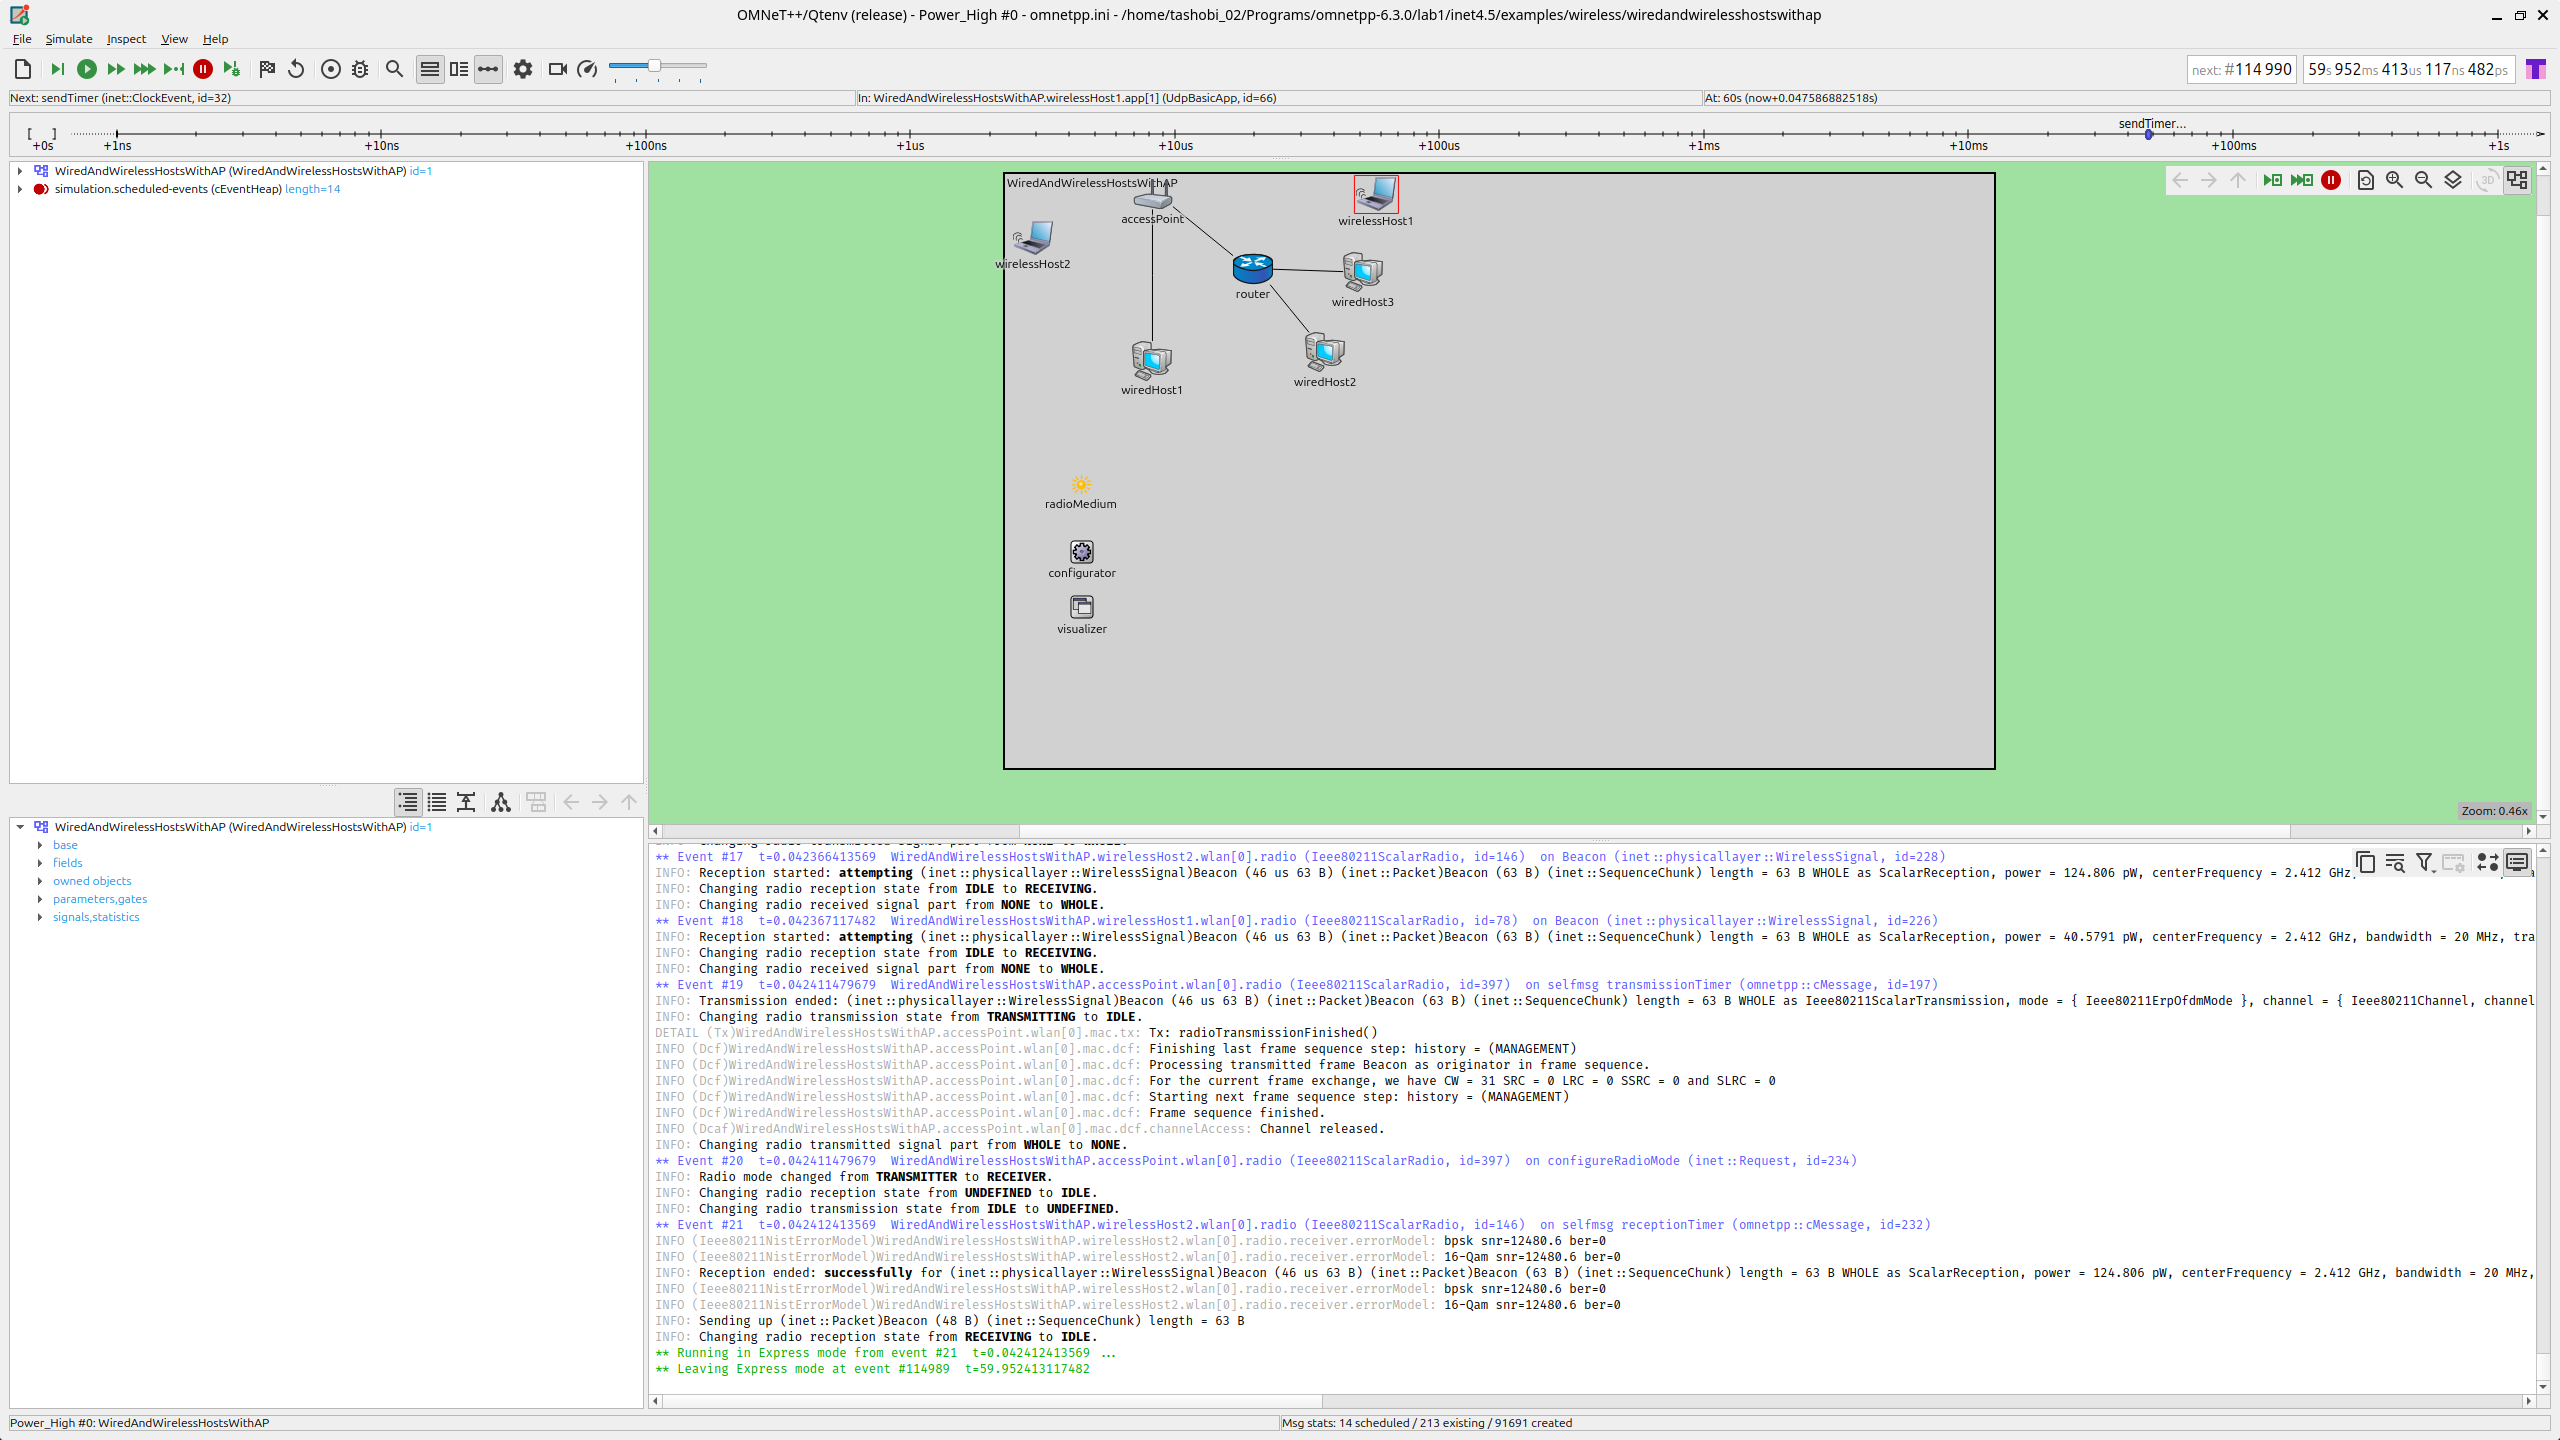
\includegraphics[width=\linewidth]{Figure/Task1_PowerHigh.png}
        \caption{Power High (100\,mW) at $t \approx 60$\,s --- link works;
                 received power $\approx -74$\,dBm at \texttt{wirelessHost1}.}
    \end{subfigure}
    \vspace{6pt}
    \begin{subfigure}{0.9\linewidth}
        \centering
        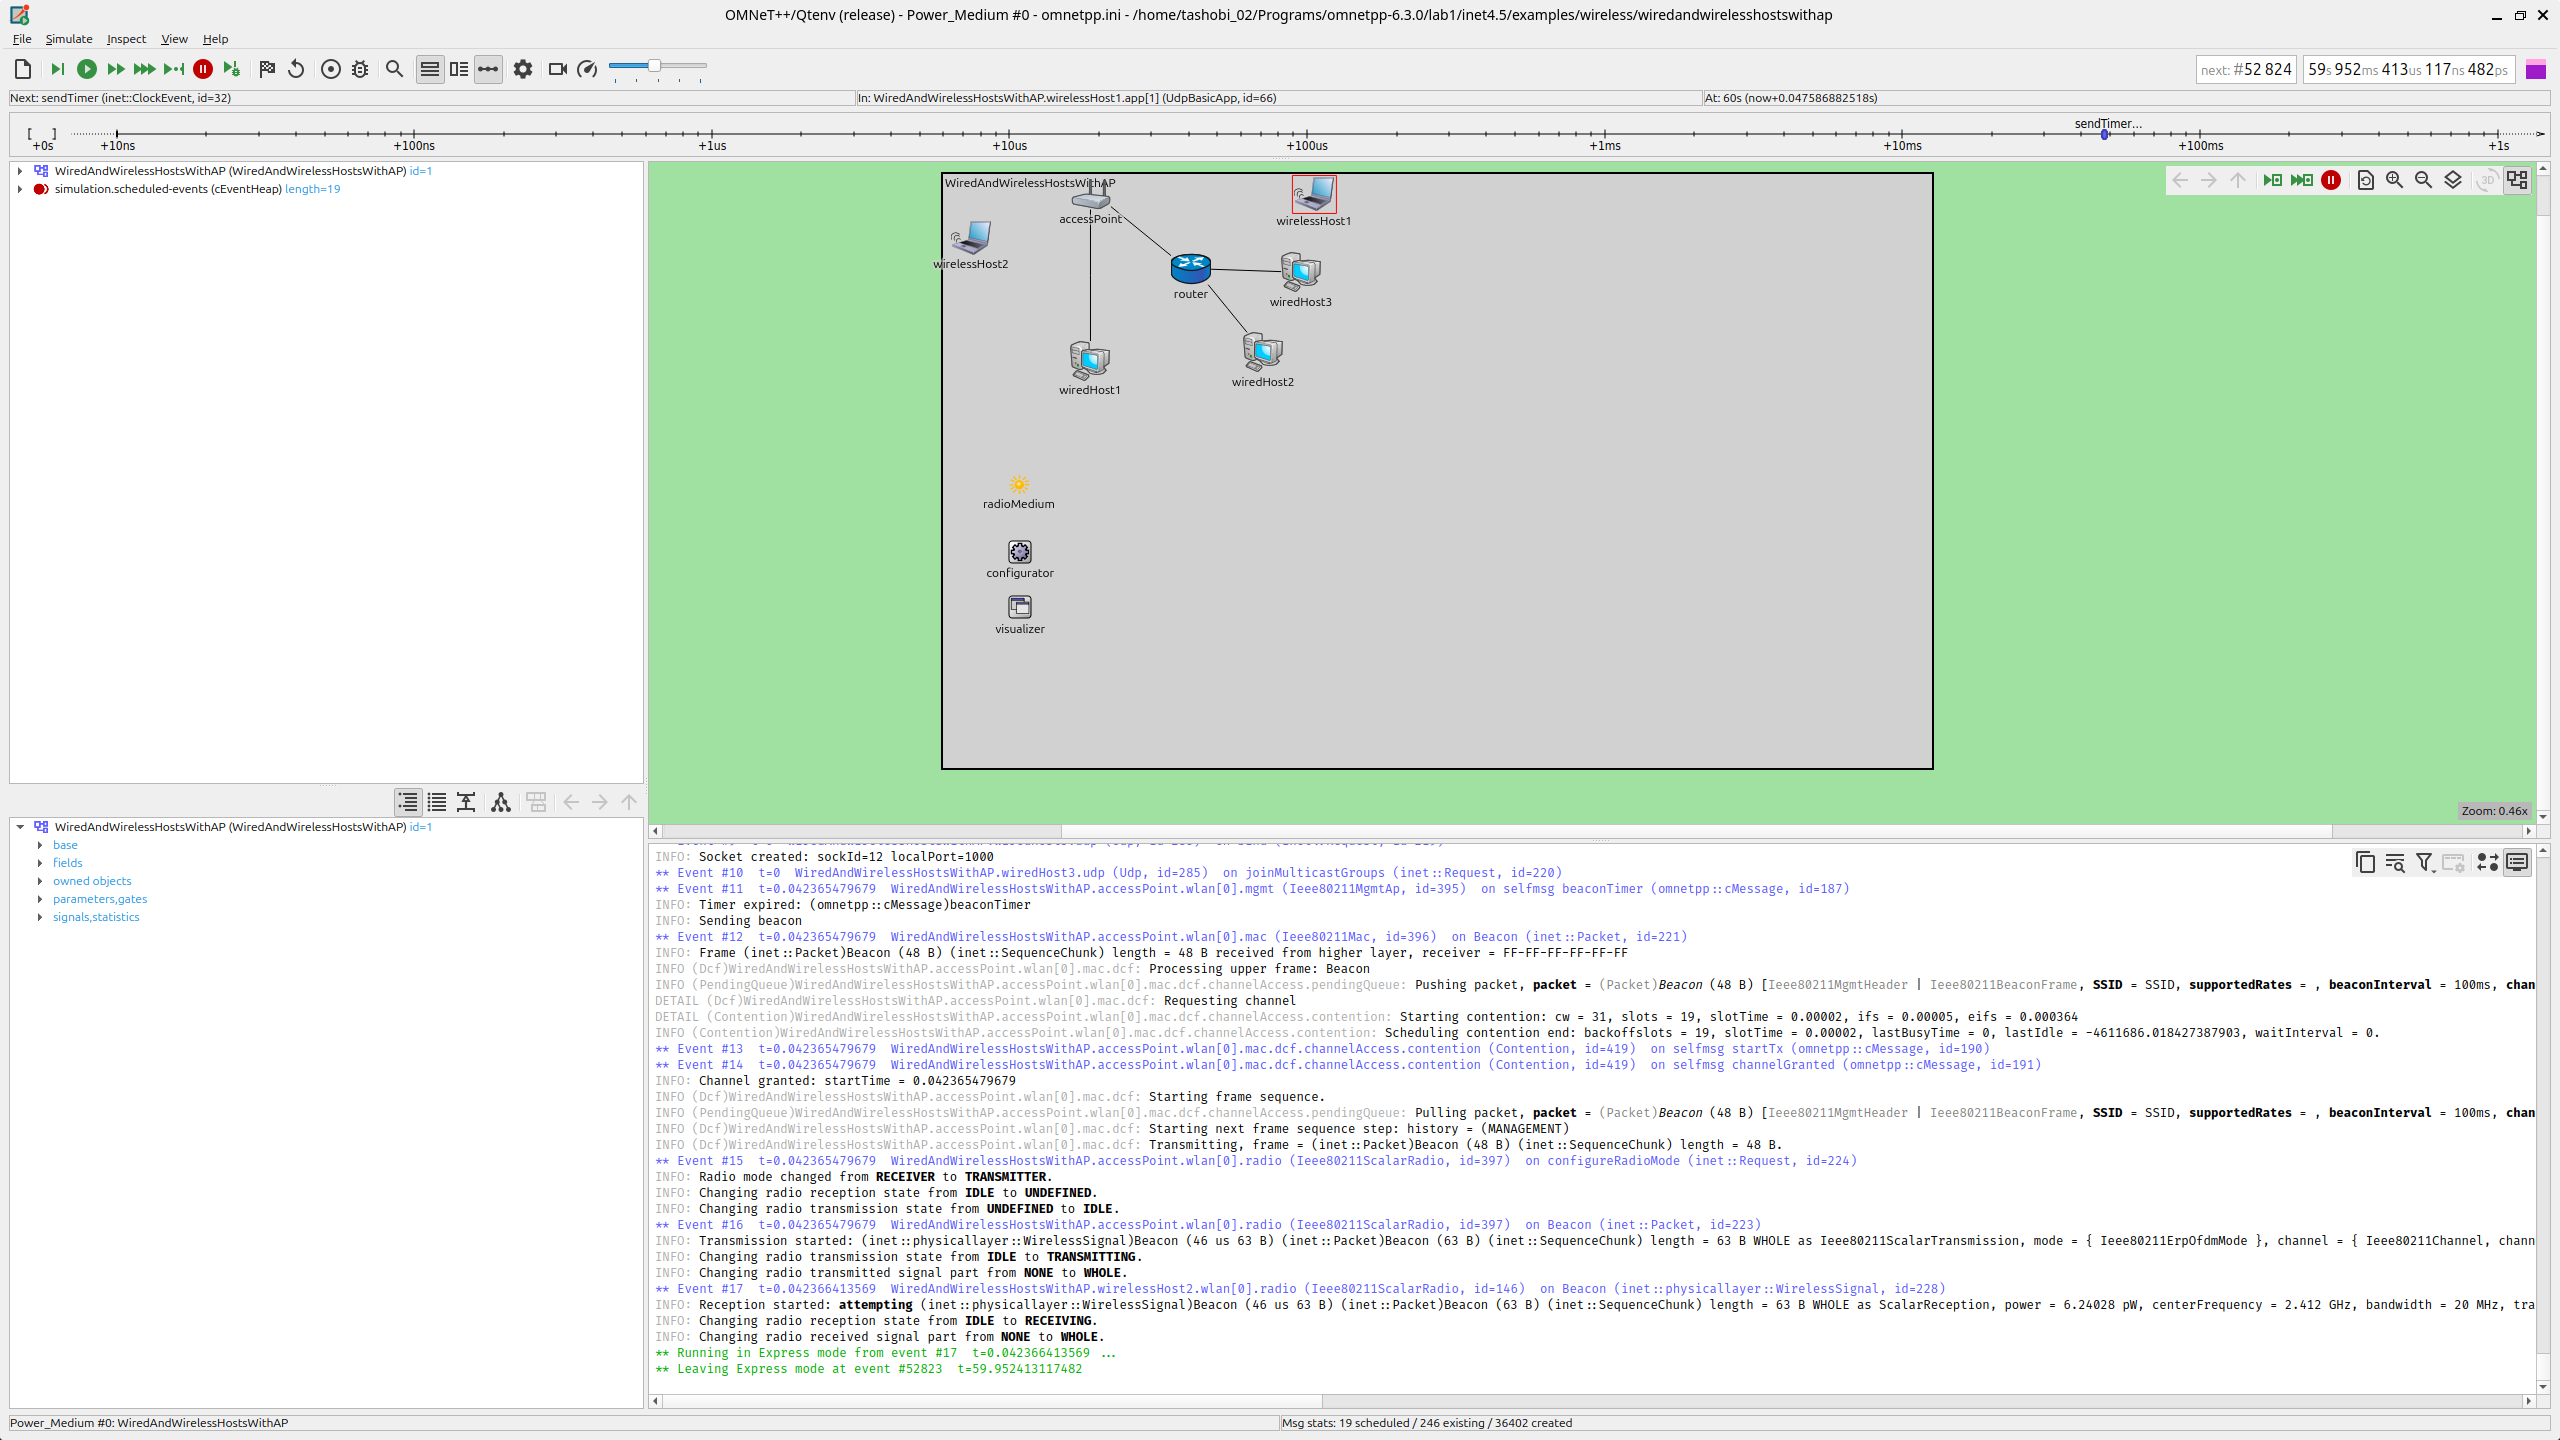
\includegraphics[width=\linewidth]{Figure/Task1_PowerMedium.png}
        \caption{Power Medium (5\,mW) at $t \approx 60$\,s --- link marginal;
                 \texttt{wirelessHost2} receives at $\approx -82$\,dBm (just above
                 sensitivity).}
    \end{subfigure}
    \vspace{6pt}
    \begin{subfigure}{0.9\linewidth}
        \centering
        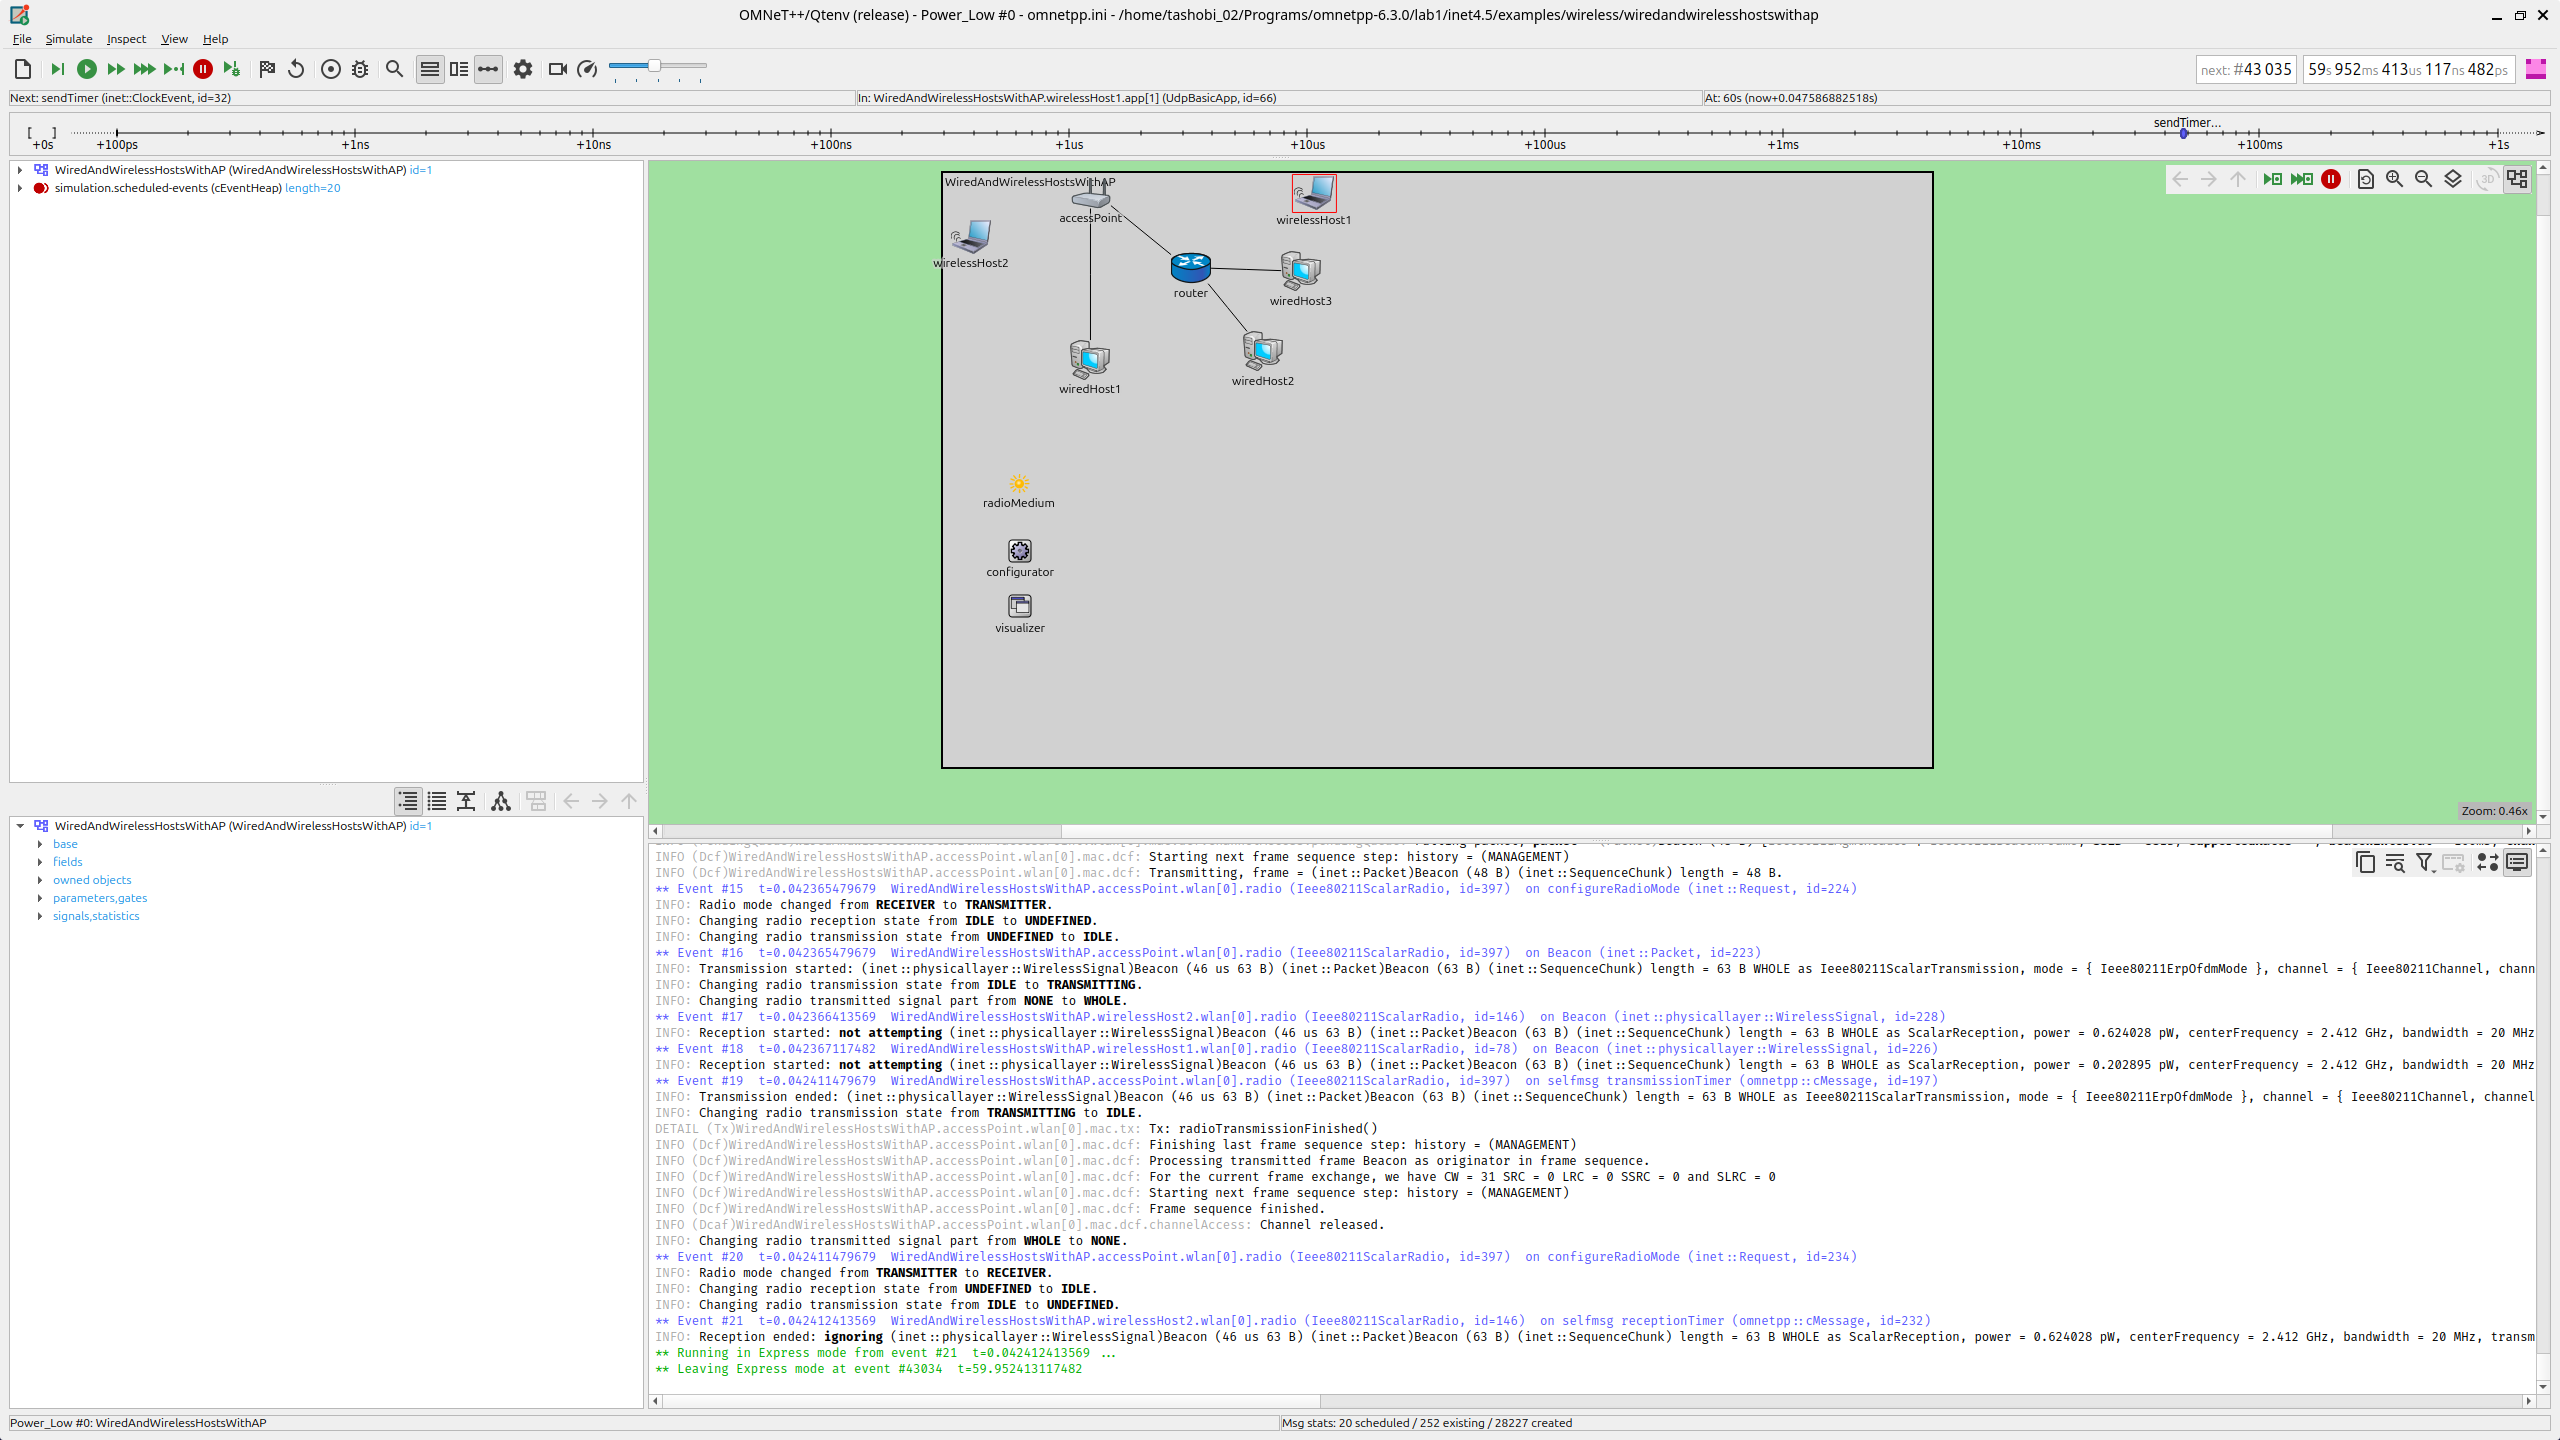
\includegraphics[width=\linewidth]{Figure/Task1_PowerLow.png}
        \caption{Power Low (0.5\,mW) at $t \approx 60$\,s --- complete wireless
                 link failure; console shows \textit{``Reception started: not
                 attempting''} at $\approx -97$\,dBm (below $-85$\,dBm
                 sensitivity).}
    \end{subfigure}
    \caption{Qtenv screenshots for Task 01.}
    \label{fig:task1}
\end{figure}

% ----------------------------------------------------------------
\subsection{Task 02: SNR Degradation and the Noise Floor}
% ----------------------------------------------------------------

\textbf{Background:} From Lecture 1, a lower signal-to-noise ratio (SNR) increases
the probability of bit errors. The noise floor in a wireless system is set by thermal
noise, interference from nearby devices, and environmental electromagnetic radiation.
In this task, the background noise level is raised progressively and the effect on
receiver SNR is observed.

\textbf{Required Modifications (INI file only):}
\begin{enumerate}
    \item \textbf{Noise\_VeryLow} -- background noise of $-120$\,dBm.
    \item \textbf{Noise\_Baseline} -- background noise of $-110$\,dBm.
    \item \textbf{Noise\_High} -- background noise of $-90$\,dBm.
    \item \textbf{Noise\_Extreme} -- background noise of $-75$\,dBm.
\end{enumerate}

\textbf{SNR Calculation Exercise:} Assume \texttt{wirelessHost1} is approximately
10\,m from the access point. Free-space path loss at 10\,m at 2.4\,GHz is
approximately 60\,dB. With transmitter power $= 20\,\text{mW} = 13\,\text{dBm}$:
\[
  P_{\text{received}} = 13\,\text{dBm} - 60\,\text{dB} = -47\,\text{dBm}
\]

\begin{table}[H]
    \centering
    \small
    \renewcommand{\arraystretch}{1.15}
    \begin{tabularx}{\linewidth}{|l|c|c|X|}
        \hline
        \textbf{Configuration} & \textbf{Noise Floor (dBm)}
            & \textbf{SNR at 10\,m (dB)} & \textbf{Expected behaviour} \\
        \hline
        Noise VeryLow  & $-120$ & $-47-(-120) = 73$ &
            54\,Mbps (64-QAM) viable; 48\,dB above the 25\,dB minimum \\
        \hline
        Noise Baseline & $-110$ & $-47-(-110) = 63$ &
            54\,Mbps viable; 38\,dB above minimum \\
        \hline
        Noise High     & $-90$  & $-47-(-90)  = 43$ &
            54\,Mbps viable; 18\,dB above minimum; slight degradation
            possible \\
        \hline
        Noise Extreme  & $-75$  & $-47-(-75)  = 28$ &
            Only 3\,dB above the 25\,dB minimum for 54\,Mbps; link highly
            unreliable. Additionally, the noise floor ($-75$\,dBm) exceeds
            the energy-detection threshold ($-85$\,dBm), causing the MAC to
            permanently detect the channel as busy --- INET refuses to
            initialise and reports an error \\
        \hline
    \end{tabularx}
    \caption{SNR calculation table for Task 02.}
    \label{tab:task2_snr}
\end{table}

\textbf{Analysis Questions:}
\begin{enumerate}

    \item \textit{In Noise Extreme, what happened to traffic from
          \texttt{wirelessHost1}? Did wired traffic between \texttt{wiredHost1}
          and \texttt{wiredHost2} also fail? Explain why or why not.}

    \textbf{Answer:}
    In the Noise\_Extreme configuration, traffic from \texttt{wirelessHost1}
    \textbf{failed completely}. Because the background noise power
    ($-75$\,dBm) exceeds the \texttt{receiver.energyDetection} threshold
    ($-85$\,dBm), the 802.11 radio permanently senses the channel as busy. As
    a result INET aborts network initialisation and displays the error:
    \textit{``Receiver is busy without any ongoing transmission, probably energy
    detection level is too low or background noise level is too high.''} The
    wireless interface never gets a chance to transmit.

    The wired link between \texttt{wiredHost1} and \texttt{wiredHost2}
    continued to work normally. Ethernet uses guided media, which is completely
    isolated from radio-frequency noise. The \texttt{backgroundNoise.power}
    parameter affects only the shared wireless radio medium and has no effect on
    Ethernet links.

    \item \textit{From Lecture 1: ``Noise distorts the signal, making it hard to
          detect correct bits.'' At which noise level does the 54\,Mbps link first
          become unreliable? Justify using the lab manual's SNR--modulation table.}

    \textbf{Answer:}
    The 54\,Mbps link (64-QAM) requires a minimum SNR of approximately 25\,dB.
    From Table~\ref{tab:task2_snr}: VeryLow gives 73\,dB, Baseline gives 63\,dB,
    and High gives 43\,dB --- all comfortably above the 25\,dB threshold. The link
    \textbf{first becomes unreliable at Noise\_Extreme} (SNR = 28\,dB), where only
    3\,dB of margin remains. Even before bit errors become dominant, the energy
    detection mechanism blocks all transmissions because the noise floor itself
    exceeds the channel-busy threshold.

    \item \textit{In Qtenv, run Noise High and Noise Extreme back to back. Describe
          any visual difference in packet animations between the two runs.}

    \textbf{Answer:}
    In \textbf{Noise\_High}, packet animations from \texttt{wirelessHost1} are still
    visible on the Qtenv canvas. The 43\,dB SNR is well above the 25\,dB minimum for
    64-QAM, so frames are decoded successfully and the wireless path operates normally,
    though with a reduced safety margin compared to the baseline.

    In \textbf{Noise\_Extreme}, no packet animations appear at all. INET raises an
    error dialog during network initialisation (\textit{``Receiver is busy without
    any ongoing transmission''}) and the simulation halts before any traffic is
    generated. The canvas remains empty. The visual contrast is stark: Noise\_High
    shows continuous wireless traffic, while Noise\_Extreme produces an immediate
    initialisation failure with a blank canvas.

    \item \textit{A real-world example from Lecture 1 is a 2.4\,GHz microwave oven
          interfering with Wi-Fi. Which of your four configurations most closely
          models this scenario? Explain your reasoning.}

    \textbf{Answer:}
    \textbf{Noise\_Extreme} ($-75$\,dBm) most closely models a microwave oven
    interfering with Wi-Fi. A microwave oven operating at approximately 2.45\,GHz
    generates broadband electromagnetic noise across the entire 2.4\,GHz ISM band
    at high power levels. Lecture 1 explicitly lists microwave ovens as a source of
    electromagnetic interference at 2.4\,GHz. Among the four configurations, the
    $-75$\,dBm noise floor best represents the severe, wideband noise that a nearby
    microwave produces, raising the effective noise floor at the receiver to the point
    where the Wi-Fi MAC can no longer access the channel.

\end{enumerate}

% ---------------------------------------------------------------
% NOTE ON SCREENSHOTS:
% Task2_Noise_High.png was uploaded but its Qtenv title bar reads
% "Noise_Baseline #0", indicating that the Noise_High run was
% accidentally captured as a second Noise_Baseline screenshot.
% The figure below uses the available files; the Noise_High
% screenshot should be re-taken from the correct configuration run.
% ---------------------------------------------------------------

\begin{figure}[H]
    \centering
    \begin{subfigure}{0.48\linewidth}
        \centering
        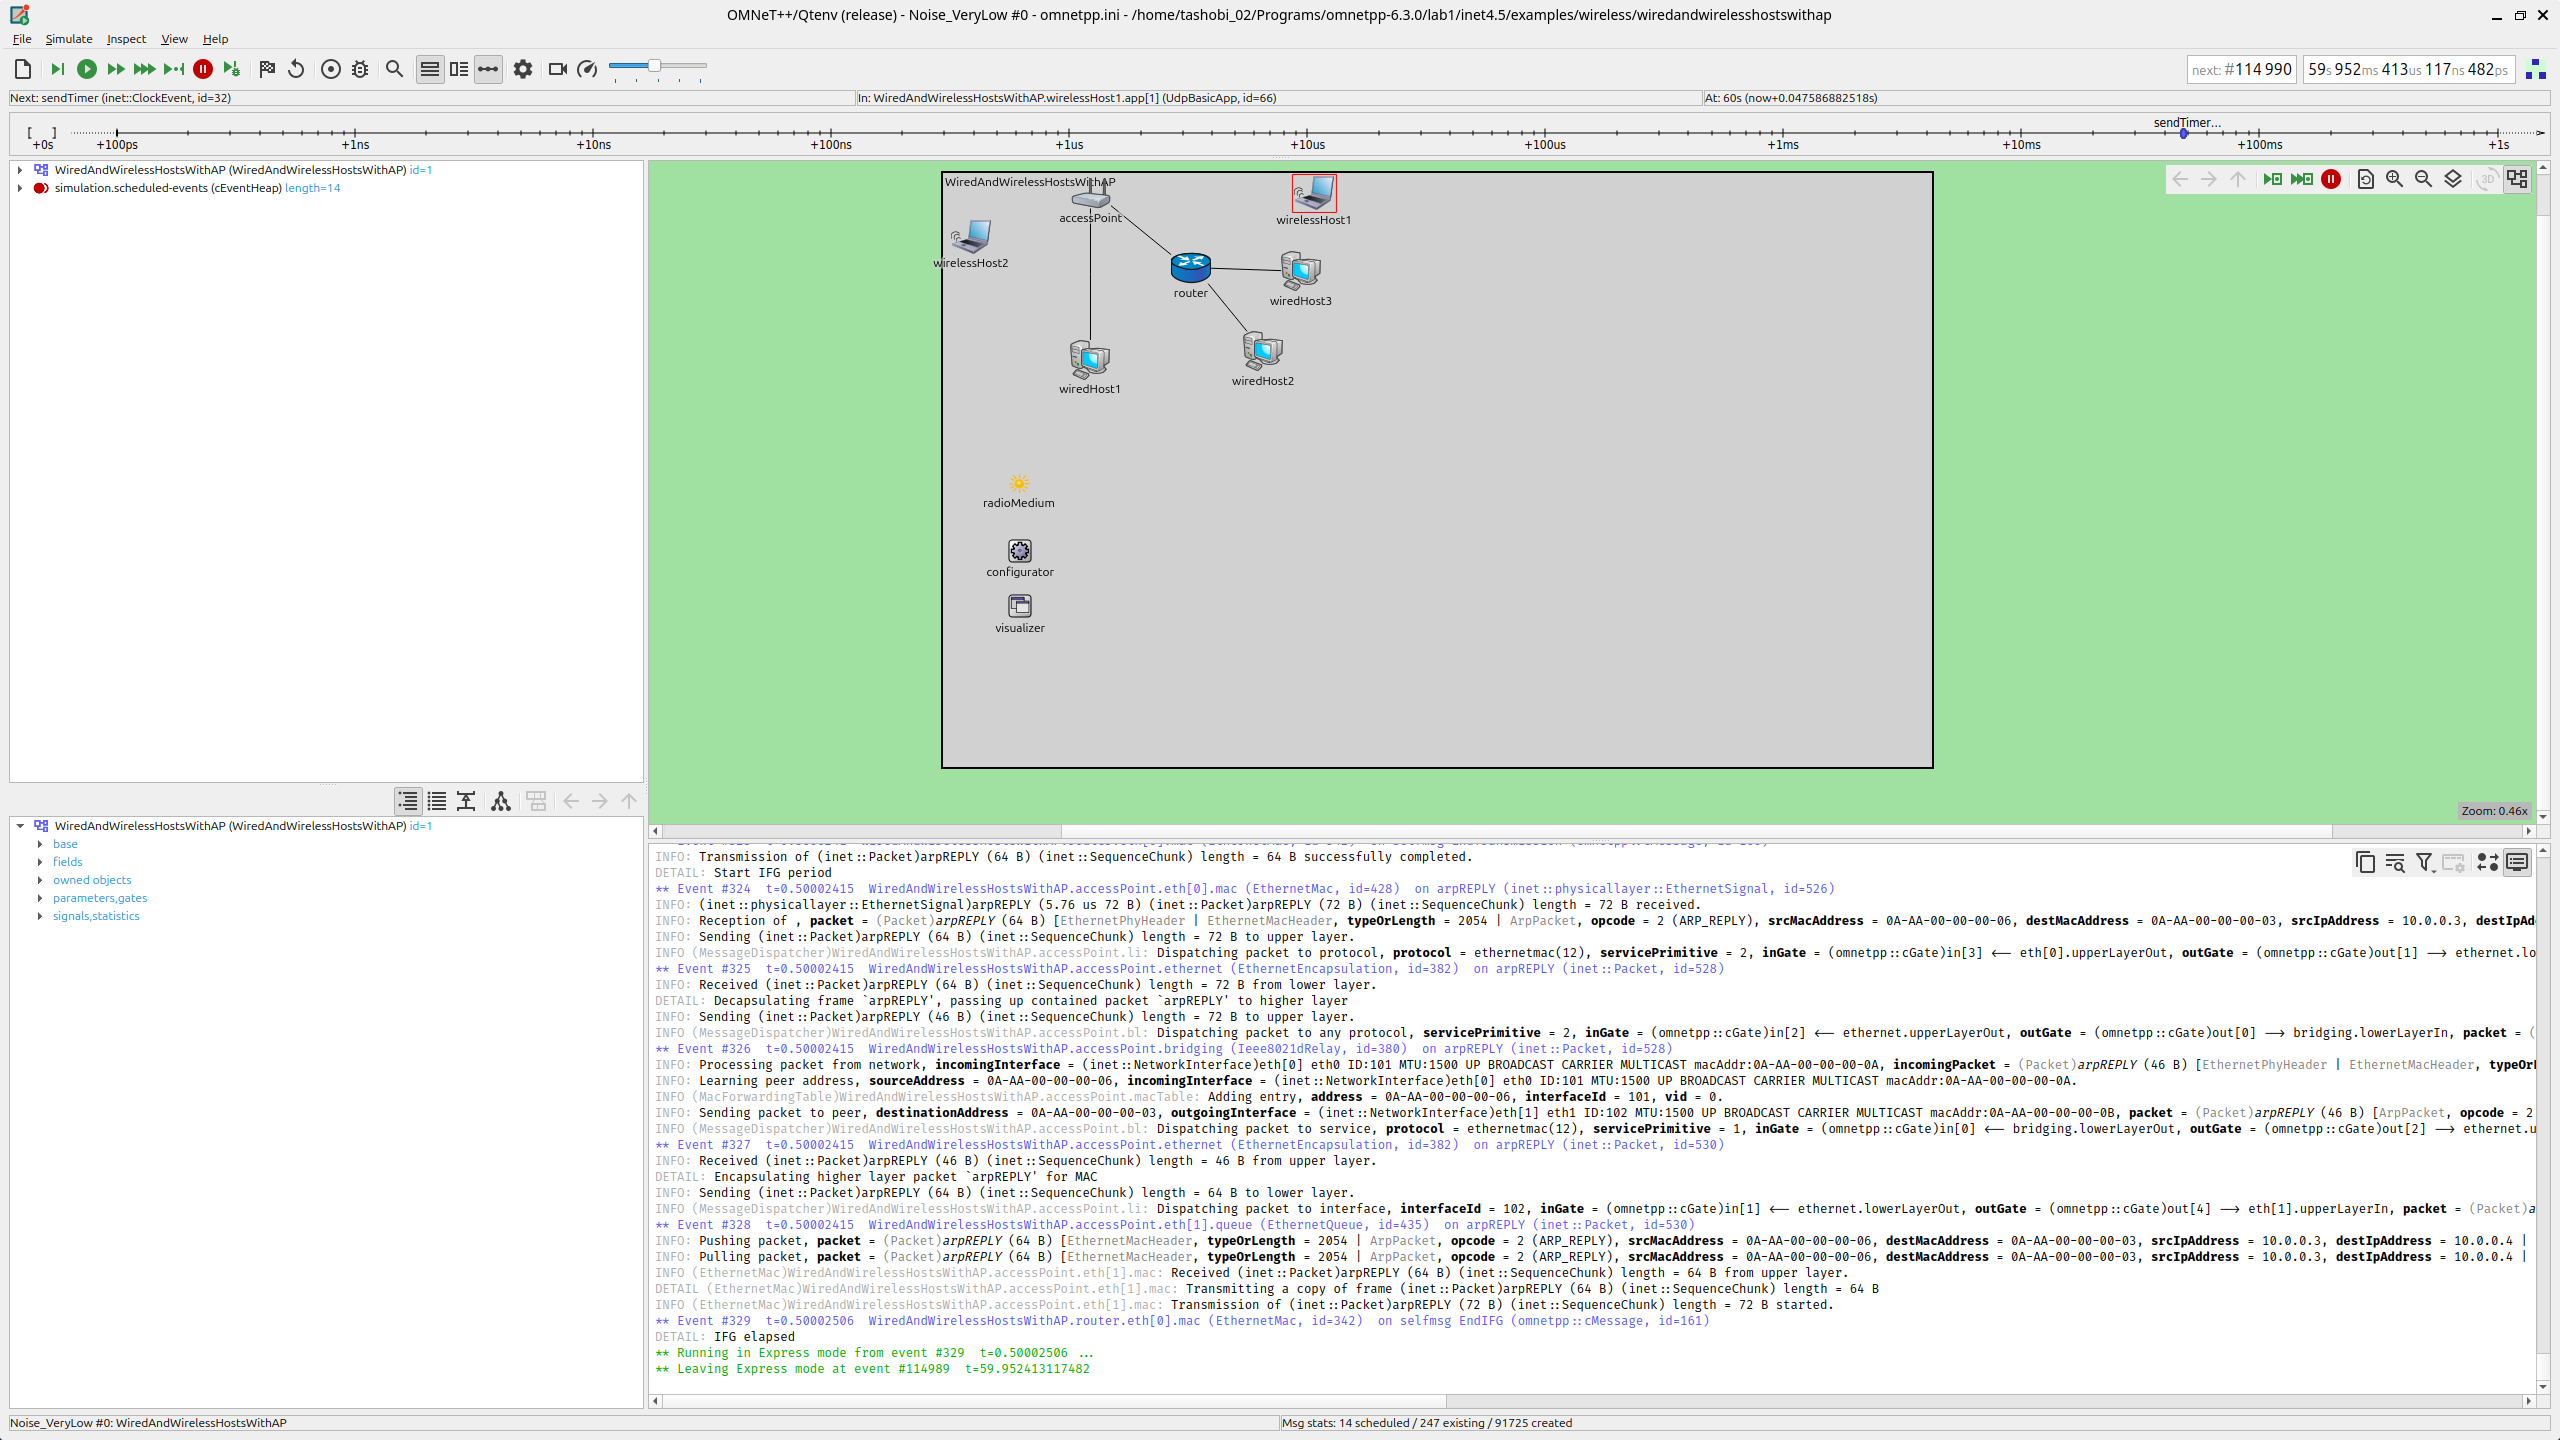
\includegraphics[width=\linewidth]{Figure/Task2_Noise_Verylow.png}
        \caption{Noise VeryLow ($-120$\,dBm) --- SNR\,=\,73\,dB, excellent link.}
    \end{subfigure}
    \hfill
    \begin{subfigure}{0.48\linewidth}
        \centering
        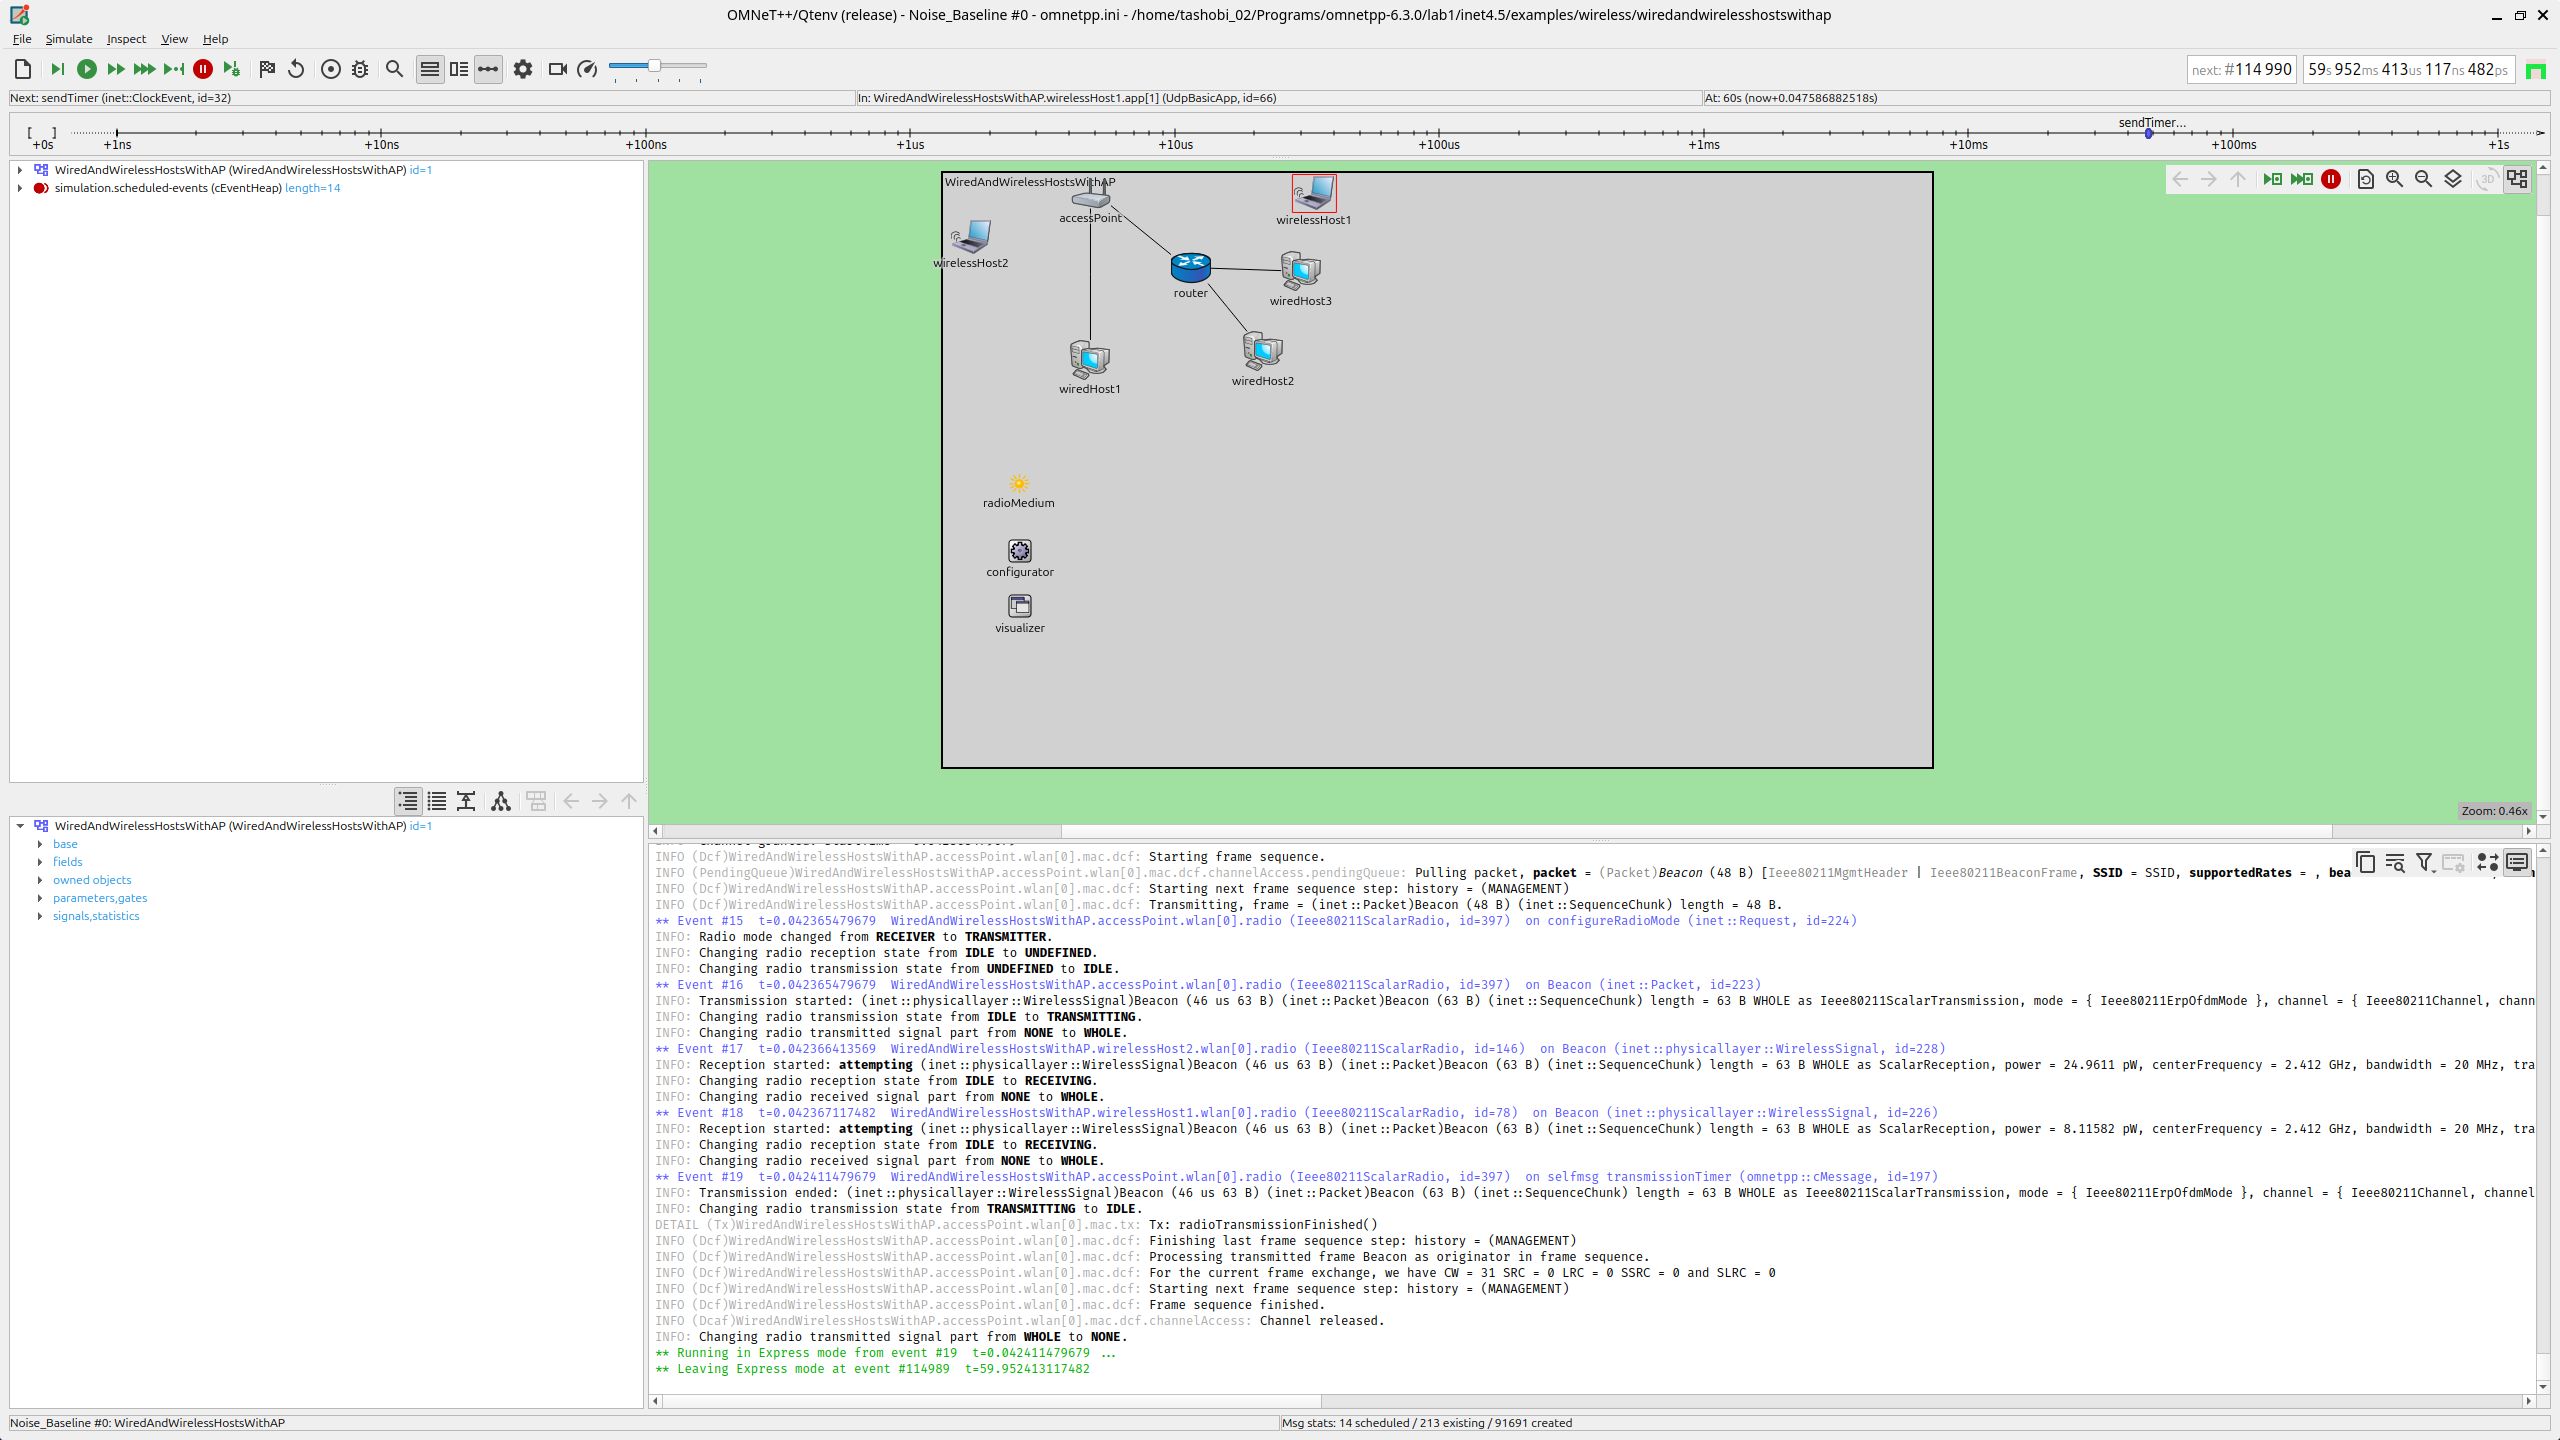
\includegraphics[width=\linewidth]{Figure/Task2_Noise_Baseline.png}
        \caption{Noise Baseline ($-110$\,dBm) --- SNR\,=\,63\,dB, healthy link.}
    \end{subfigure}

    \vspace{6pt}

    \begin{subfigure}{0.48\linewidth}
        \centering
        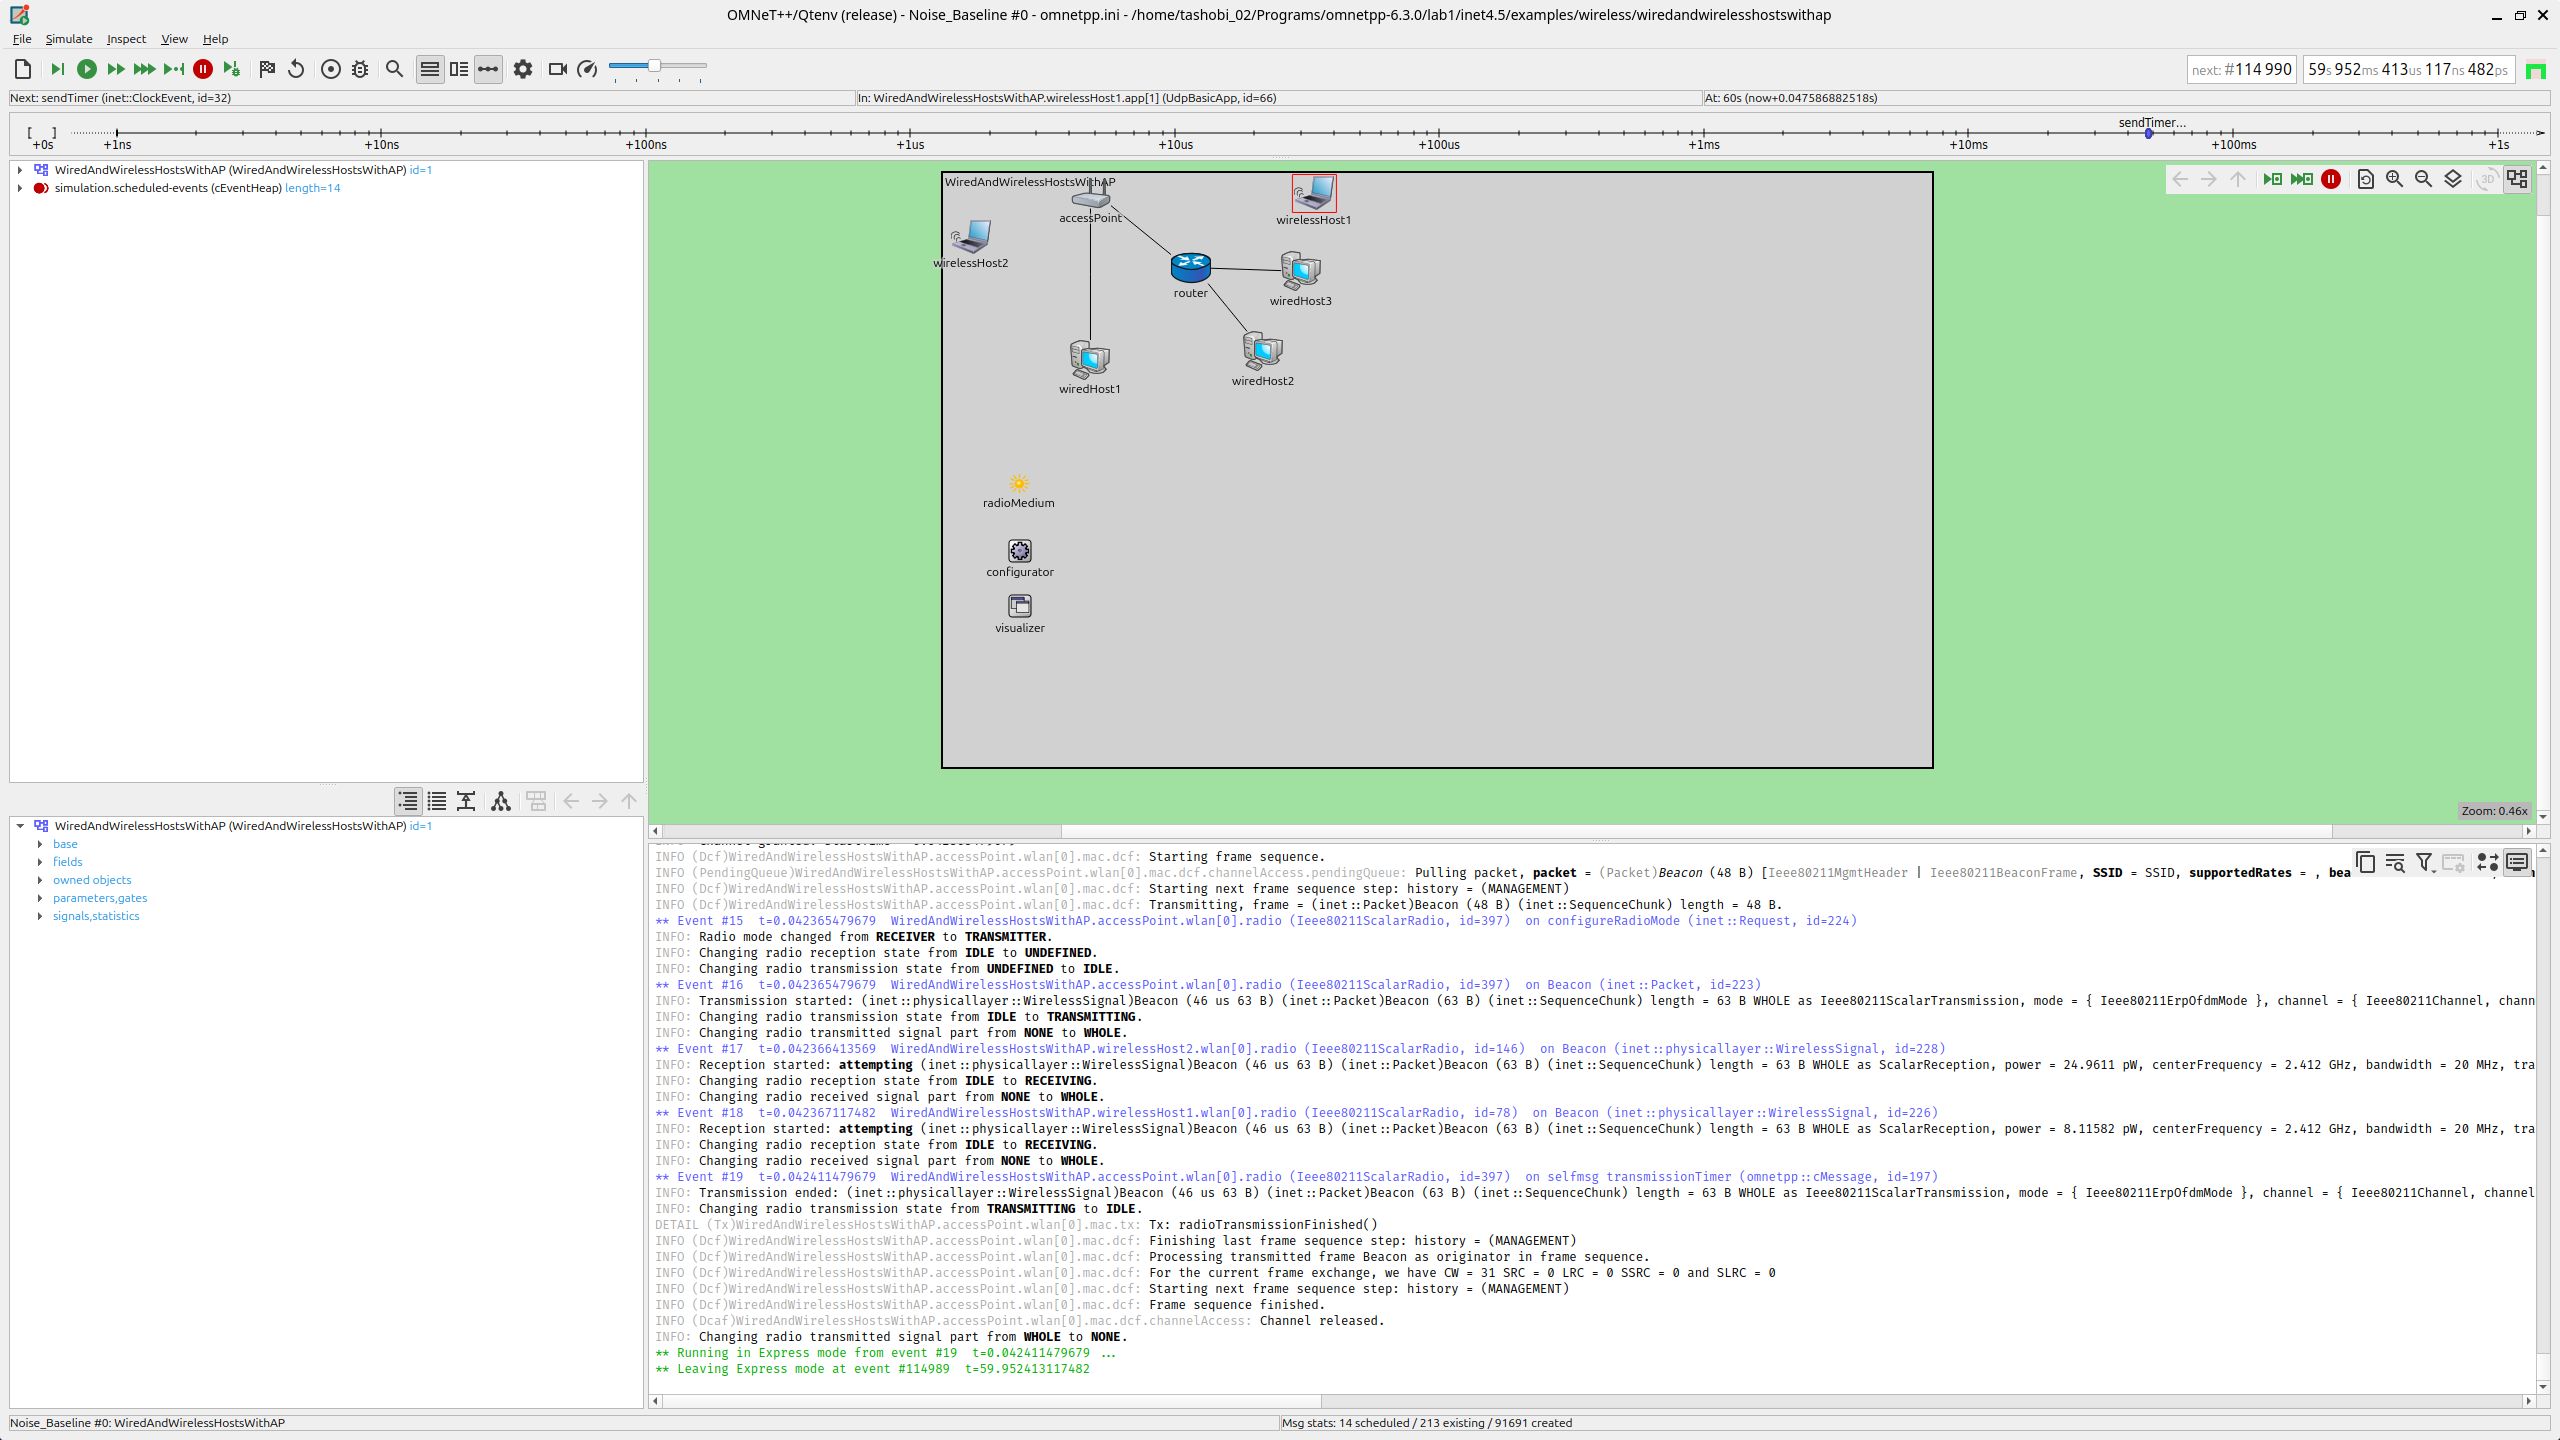
\includegraphics[width=\linewidth]{Figure/Task2_Noise_High.png}
        \caption{Noise High ($-90$\,dBm) --- SNR\,=\,43\,dB; link still operational.
                 \textit{Note: screenshot title bar shows Noise\_Baseline; the
                 Noise\_High run should be re-captured.}}
    \end{subfigure}
    \hfill
    \begin{subfigure}{0.48\linewidth}
        \centering
        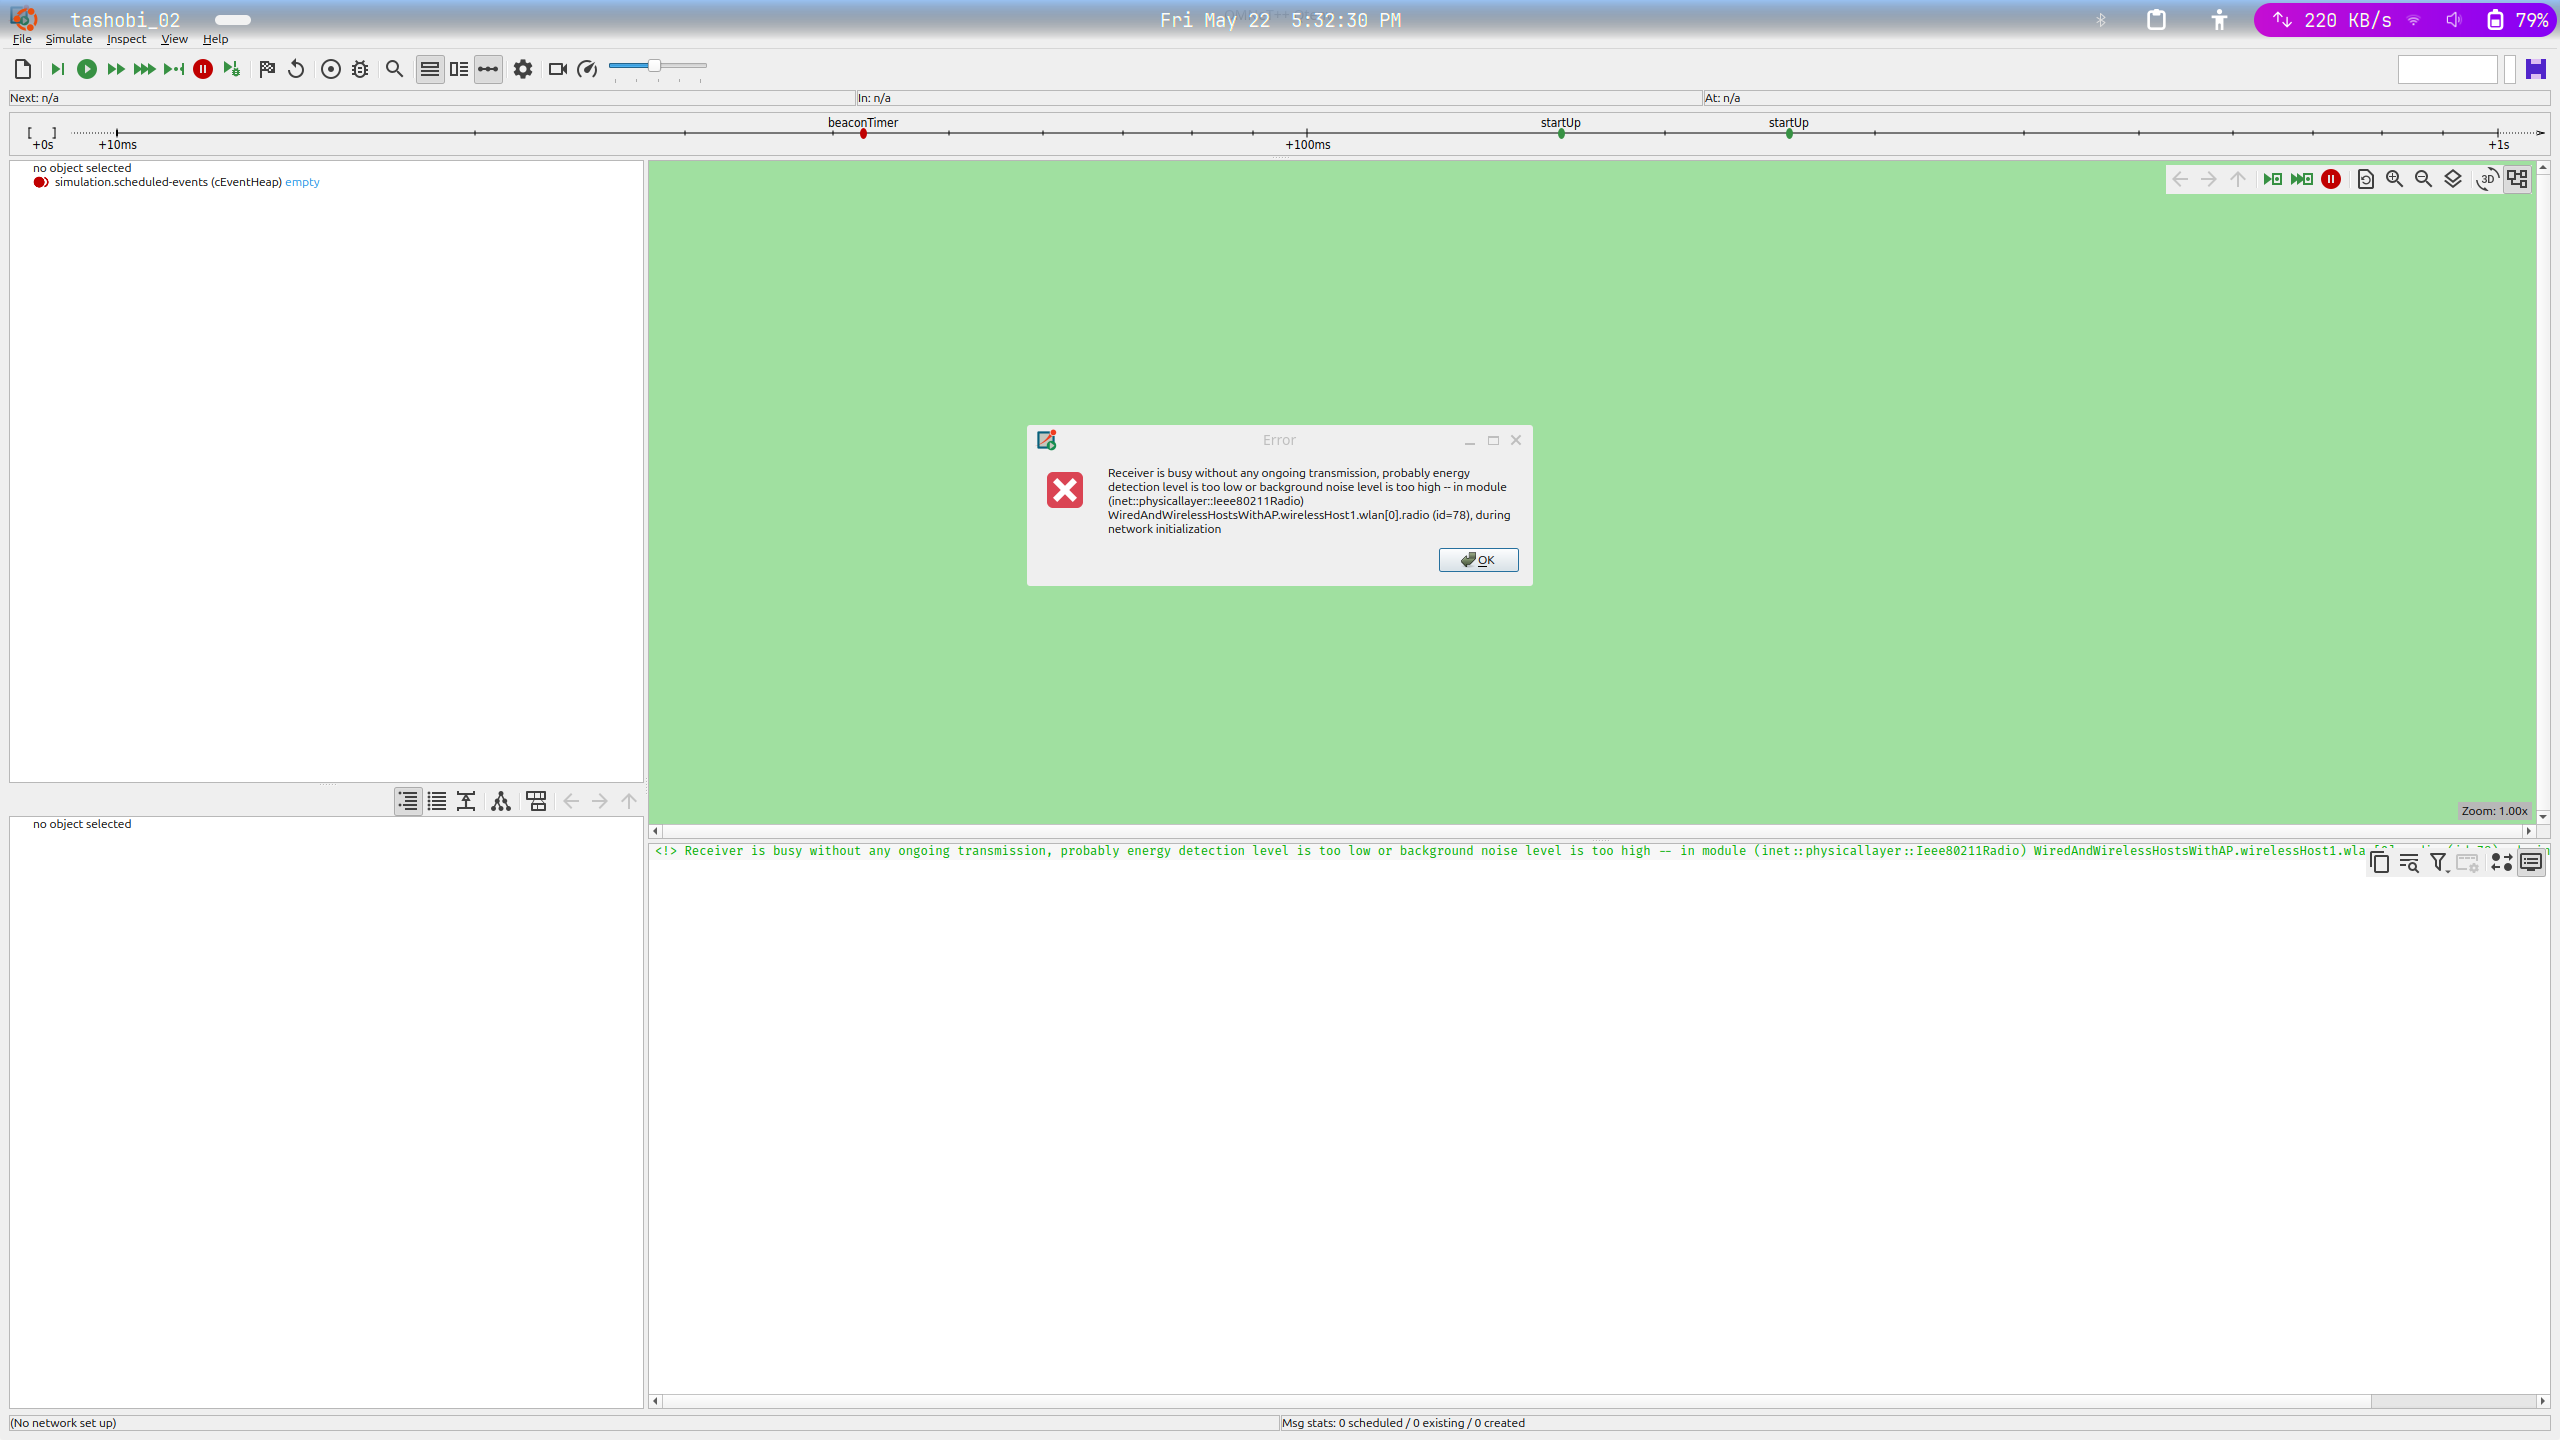
\includegraphics[width=\linewidth]{Figure/Task2_Noise_Extreme.png}
        \caption{Noise Extreme ($-75$\,dBm) --- INET initialisation error; noise
                 exceeds energyDetection threshold, wireless link cannot start.}
    \end{subfigure}
    \caption{Qtenv screenshots for Task 02.}
    \label{fig:task2}
\end{figure}

% ----------------------------------------------------------------
\subsection{Task 03: Path Loss Model Comparison}
% ----------------------------------------------------------------

\textbf{Background:} In Lecture 1, signal power in free space falls as $1/d^{2}$,
but in real environments the decay can be more severe due to reflections, diffraction,
and scattering. The LogNormal Shadowing model captures random variations in signal
strength caused by obstacles and environmental clutter, while the path loss exponent
$\alpha$ controls the average rate of decay. In this task, different values of
$\alpha$ are used to observe how the effective range and packet delivery change in
realistic environments.

\textbf{Required Modifications (INI file only):}
\begin{enumerate}
    \item \textbf{PathLoss\_FreeSpace} -- \texttt{FreeSpacePathLoss} model.
    \item \textbf{Multipath\_Study} -- \texttt{LogNormalShadowing} model with
          $\alpha = 3.5$.
    \item \textbf{PathLoss\_EdgeOfCoverage} -- \texttt{LogNormalShadowing} model
          with $\alpha = 3.5$, transmitter power reduced to 5\,mW, and receiver
          sensitivity set to $-85$\,dBm.
\end{enumerate}

\textbf{Analysis Questions:}
\begin{enumerate}

    \item \textit{If a device at 20\,m receives $-60$\,dBm under free space,
          estimate the expected received power at 40\,m using $\alpha = 3.5$
          (ignore random shadowing).}

    \textbf{Answer:}
    When distance doubles from 20\,m to 40\,m, the additional path loss with
    exponent $\alpha = 3.5$ is:
    \[
      \Delta\mathrm{PL}
        = 10\cdot\alpha\cdot\log_{10}\!\left(\frac{40}{20}\right)
        = 10 \times 3.5 \times \log_{10}(2)
        \approx 35 \times 0.3010
        \approx 10.54\,\text{dB}.
    \]
    The received power at 40\,m is therefore approximately
    $-60 - 10.54 = \mathbf{-70.5}$\,\textbf{dBm}.

    For comparison, under free space ($\alpha = 2$) the same doubling would
    add only 6.02\,dB, giving $-66$\,dBm. The LogNormal model predicts a
    4.5\,dBm additional loss at the same distance, reflecting faster decay in
    obstructed environments.

    \item \textit{Compare the PathLoss\_FreeSpace and Multipath\_Study runs. Did
          you observe any difference in packet delivery from \texttt{wirelessHost1}?
          If not, explain why.}

    \textbf{Answer:}
    At the short node distances used in this simulation topology, packet delivery
    from \texttt{wirelessHost1} is visually identical in both
    PathLoss\_FreeSpace and Multipath\_Study. Both runs show a healthy link with
    no visible drops. The reason is that the nodes are placed close to the access
    point relative to the theoretical maximum range. Even with the steeper
    $\alpha = 3.5$ decay, the link still has sufficient margin so that the
    LogNormal random shadowing does not degrade delivery measurably at these
    distances. A meaningful difference would only appear if the nodes were placed
    closer to the coverage edge (approaching or beyond the maximum usable range).

    \item \textit{In PathLoss\_EdgeOfCoverage, describe what happened to traffic
          from \texttt{wirelessHost1}. Was it completely lost or intermittent? How
          does shadowing contribute to variability in reception?}

    \textbf{Answer:}
    In the PathLoss\_EdgeOfCoverage configuration, the wireless link suffered
    \textbf{complete failure}. The Qtenv console log shows the message
    \textit{``Reception started: not attempting''} for incoming frames at
    \texttt{wirelessHost1.wlan[0].radio}, with a measured received power of
    approximately $0.00171$\,pW\,$\approx -118$\,dBm. This is approximately
    33\,dB below the receiver sensitivity threshold of $-85$\,dBm. At this
    power deficit, no amount of favourable random shadowing variation (typical
    standard deviation $\approx 8$--$10$\,dB) can lift the signal above the
    sensitivity floor, so reception is never attempted and the link is
    permanently inactive rather than intermittent.

    Shadowing would contribute variability if the node were positioned much
    closer to the coverage boundary, where the mean received power fluctuates
    above and below the sensitivity threshold. In that scenario, some
    shadowing realisations would permit reception while others would not,
    producing the intermittent behaviour characteristic of a device at the
    edge of coverage.

    \item \textit{Which of the three propagation mechanisms from Lecture 1 does
          the LogNormal Shadowing model implicitly capture, and which does it
          ignore? What environment is the model most appropriate for?}

    \textbf{Answer:}
    \textbf{Implicitly captured:} The LogNormal Shadowing model captures
    large-scale, slow-varying signal attenuation caused by obstacles and clutter.
    This is associated with \textit{diffraction} around large objects and
    \textit{scattering} from environmental clutter, both of which contribute to
    the average excess path loss encoded in the exponent $\alpha$ and to the
    log-normal random variable that represents shadowing variation.

    \textbf{Ignored:} The model does not capture fast multipath \textit{fading}
    caused by multiple reflected copies of the signal arriving with different
    phases and delays. Reflection produces rapid, frequency-selective fluctuations
    in received power (Rayleigh or Ricean fading) that the LogNormal model does
    not represent.

    \textbf{Most appropriate for:} Outdoor urban and suburban environments with
    moderate obstructions --- city streets, open campuses, or outdoor hotspot
    deployments --- where large-scale shadowing dominates and the receiver is
    stationary or slow-moving.

\end{enumerate}

\begin{figure}[H]
    \centering
    \begin{subfigure}{0.9\linewidth}
        \centering
        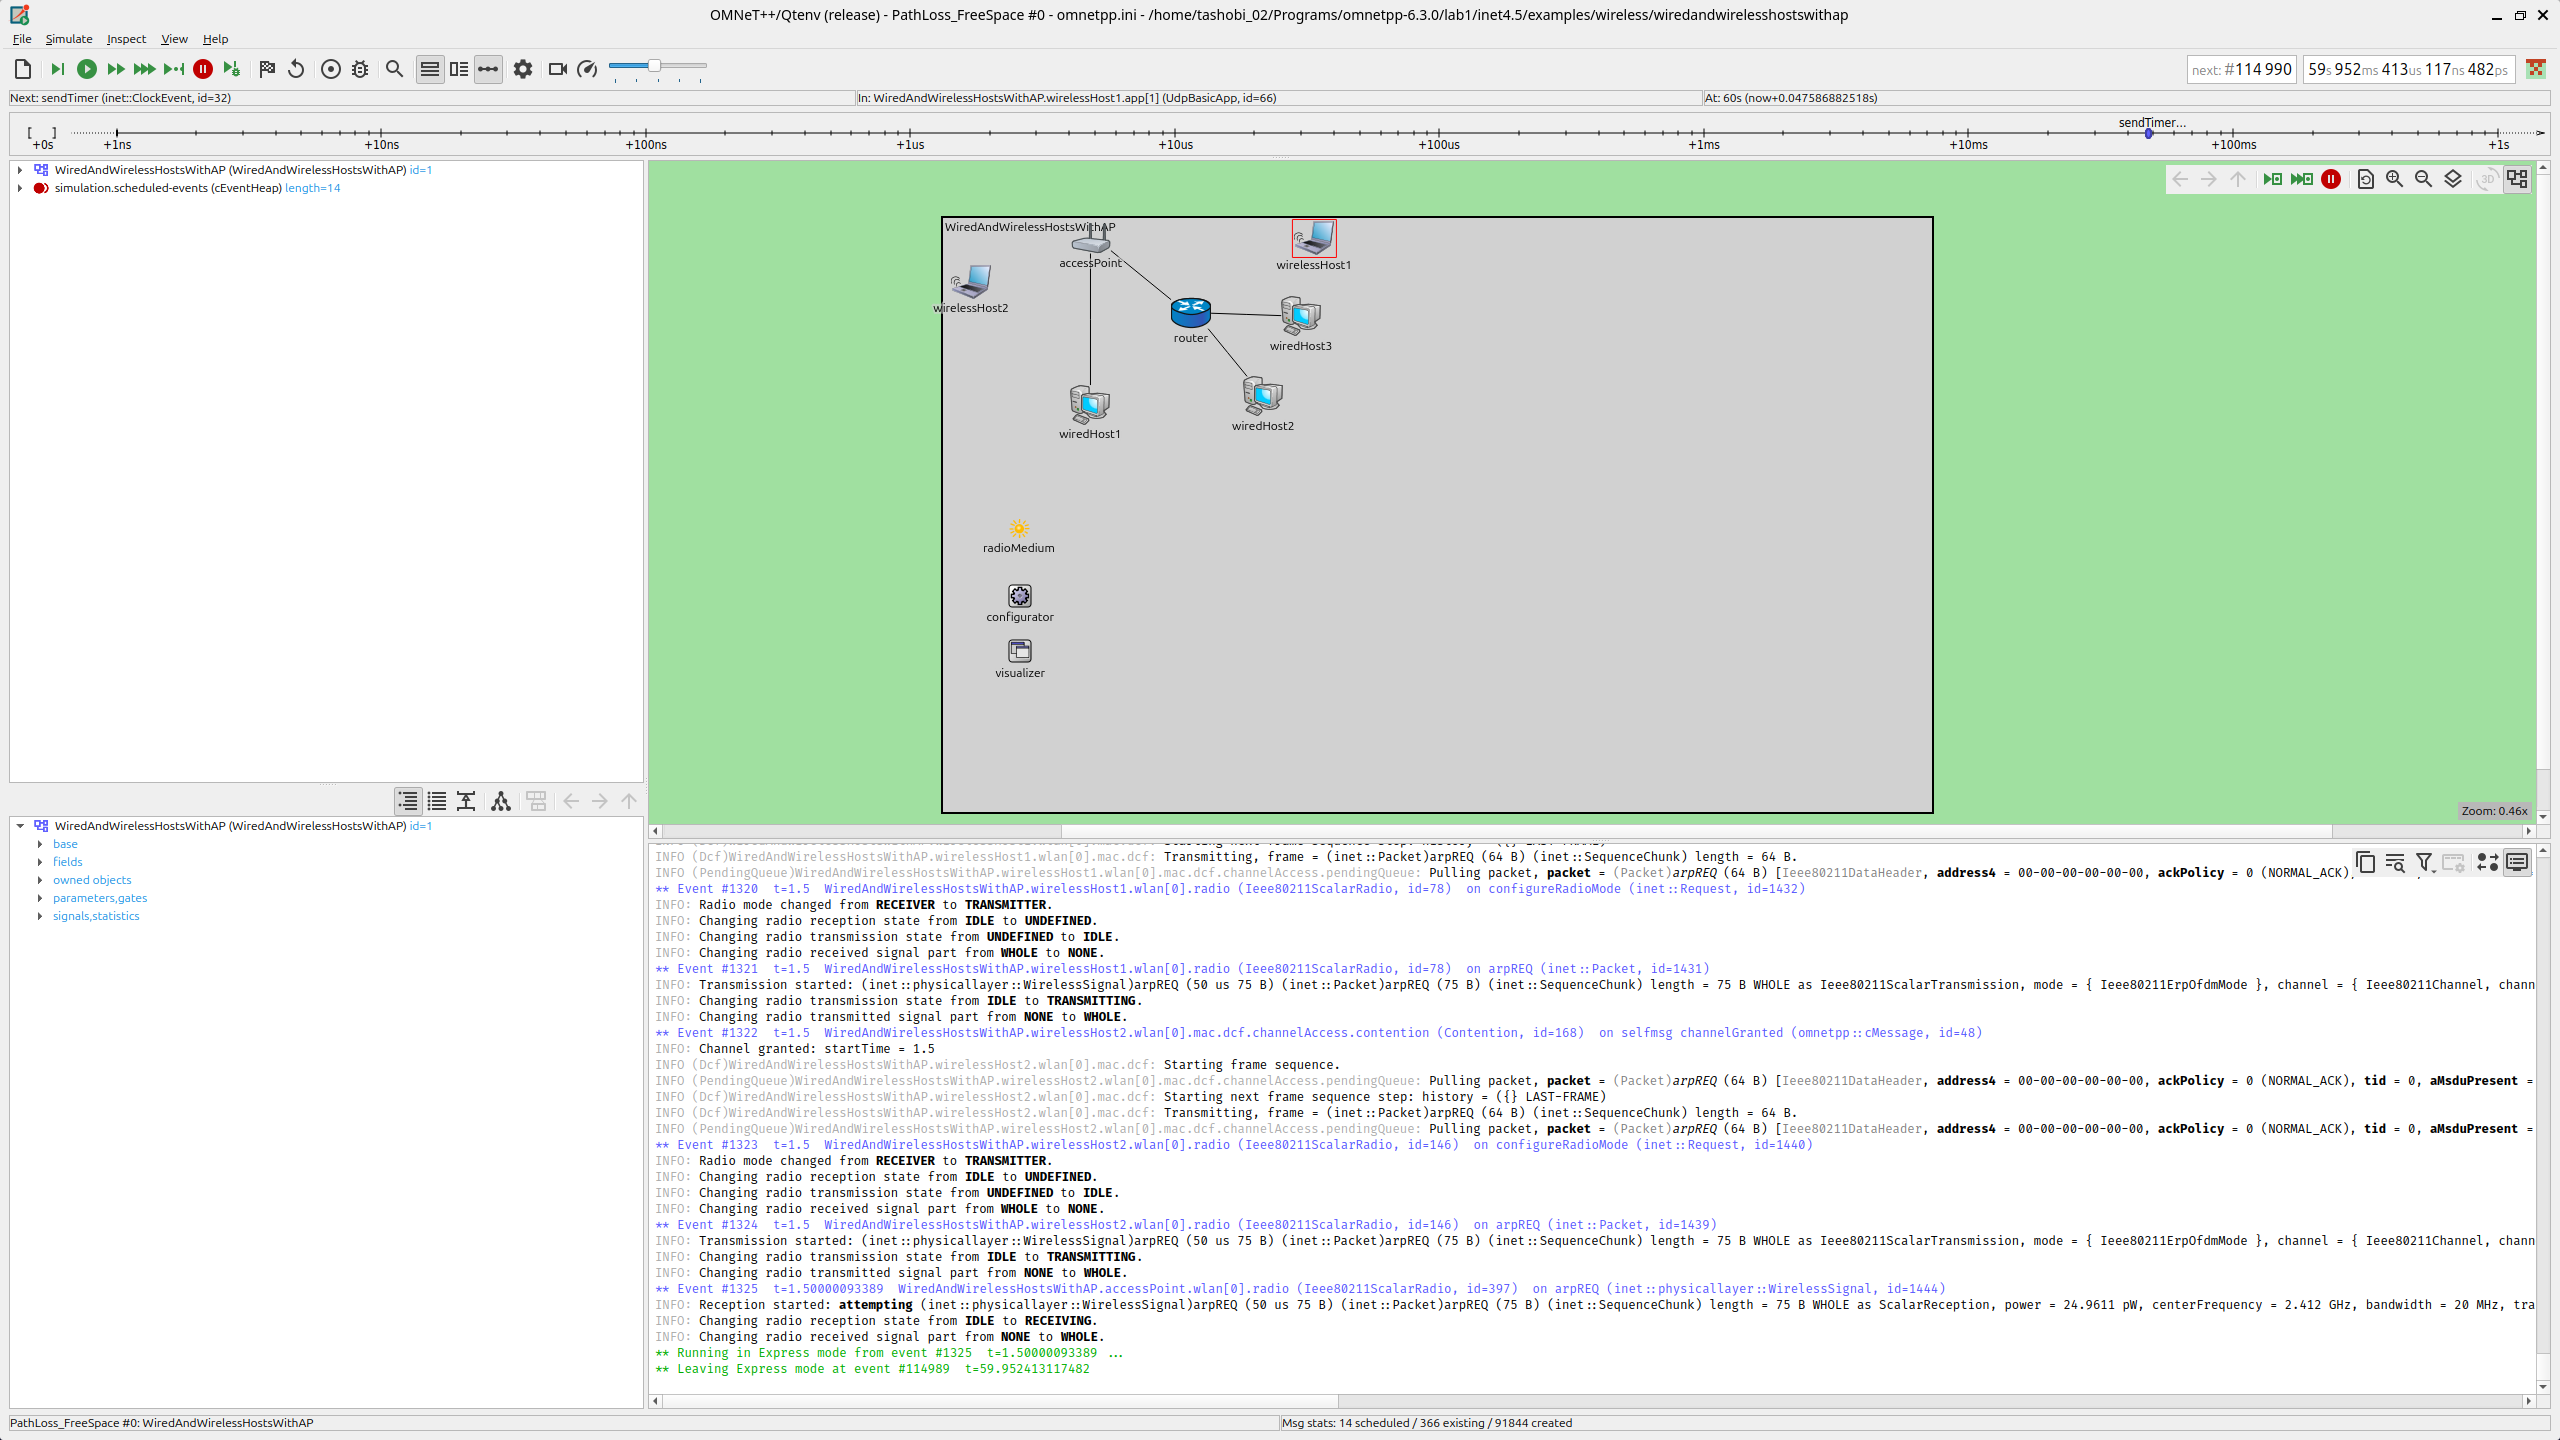
\includegraphics[width=\linewidth]{Figure/Task3_PathLoss_FreeSpace.png}
        \caption{PathLoss\_FreeSpace at $t \approx 60$\,s --- ideal 1/$d^{2}$
                 decay, link operates normally.}
    \end{subfigure}
    \vspace{6pt}
    \begin{subfigure}{0.9\linewidth}
        \centering
        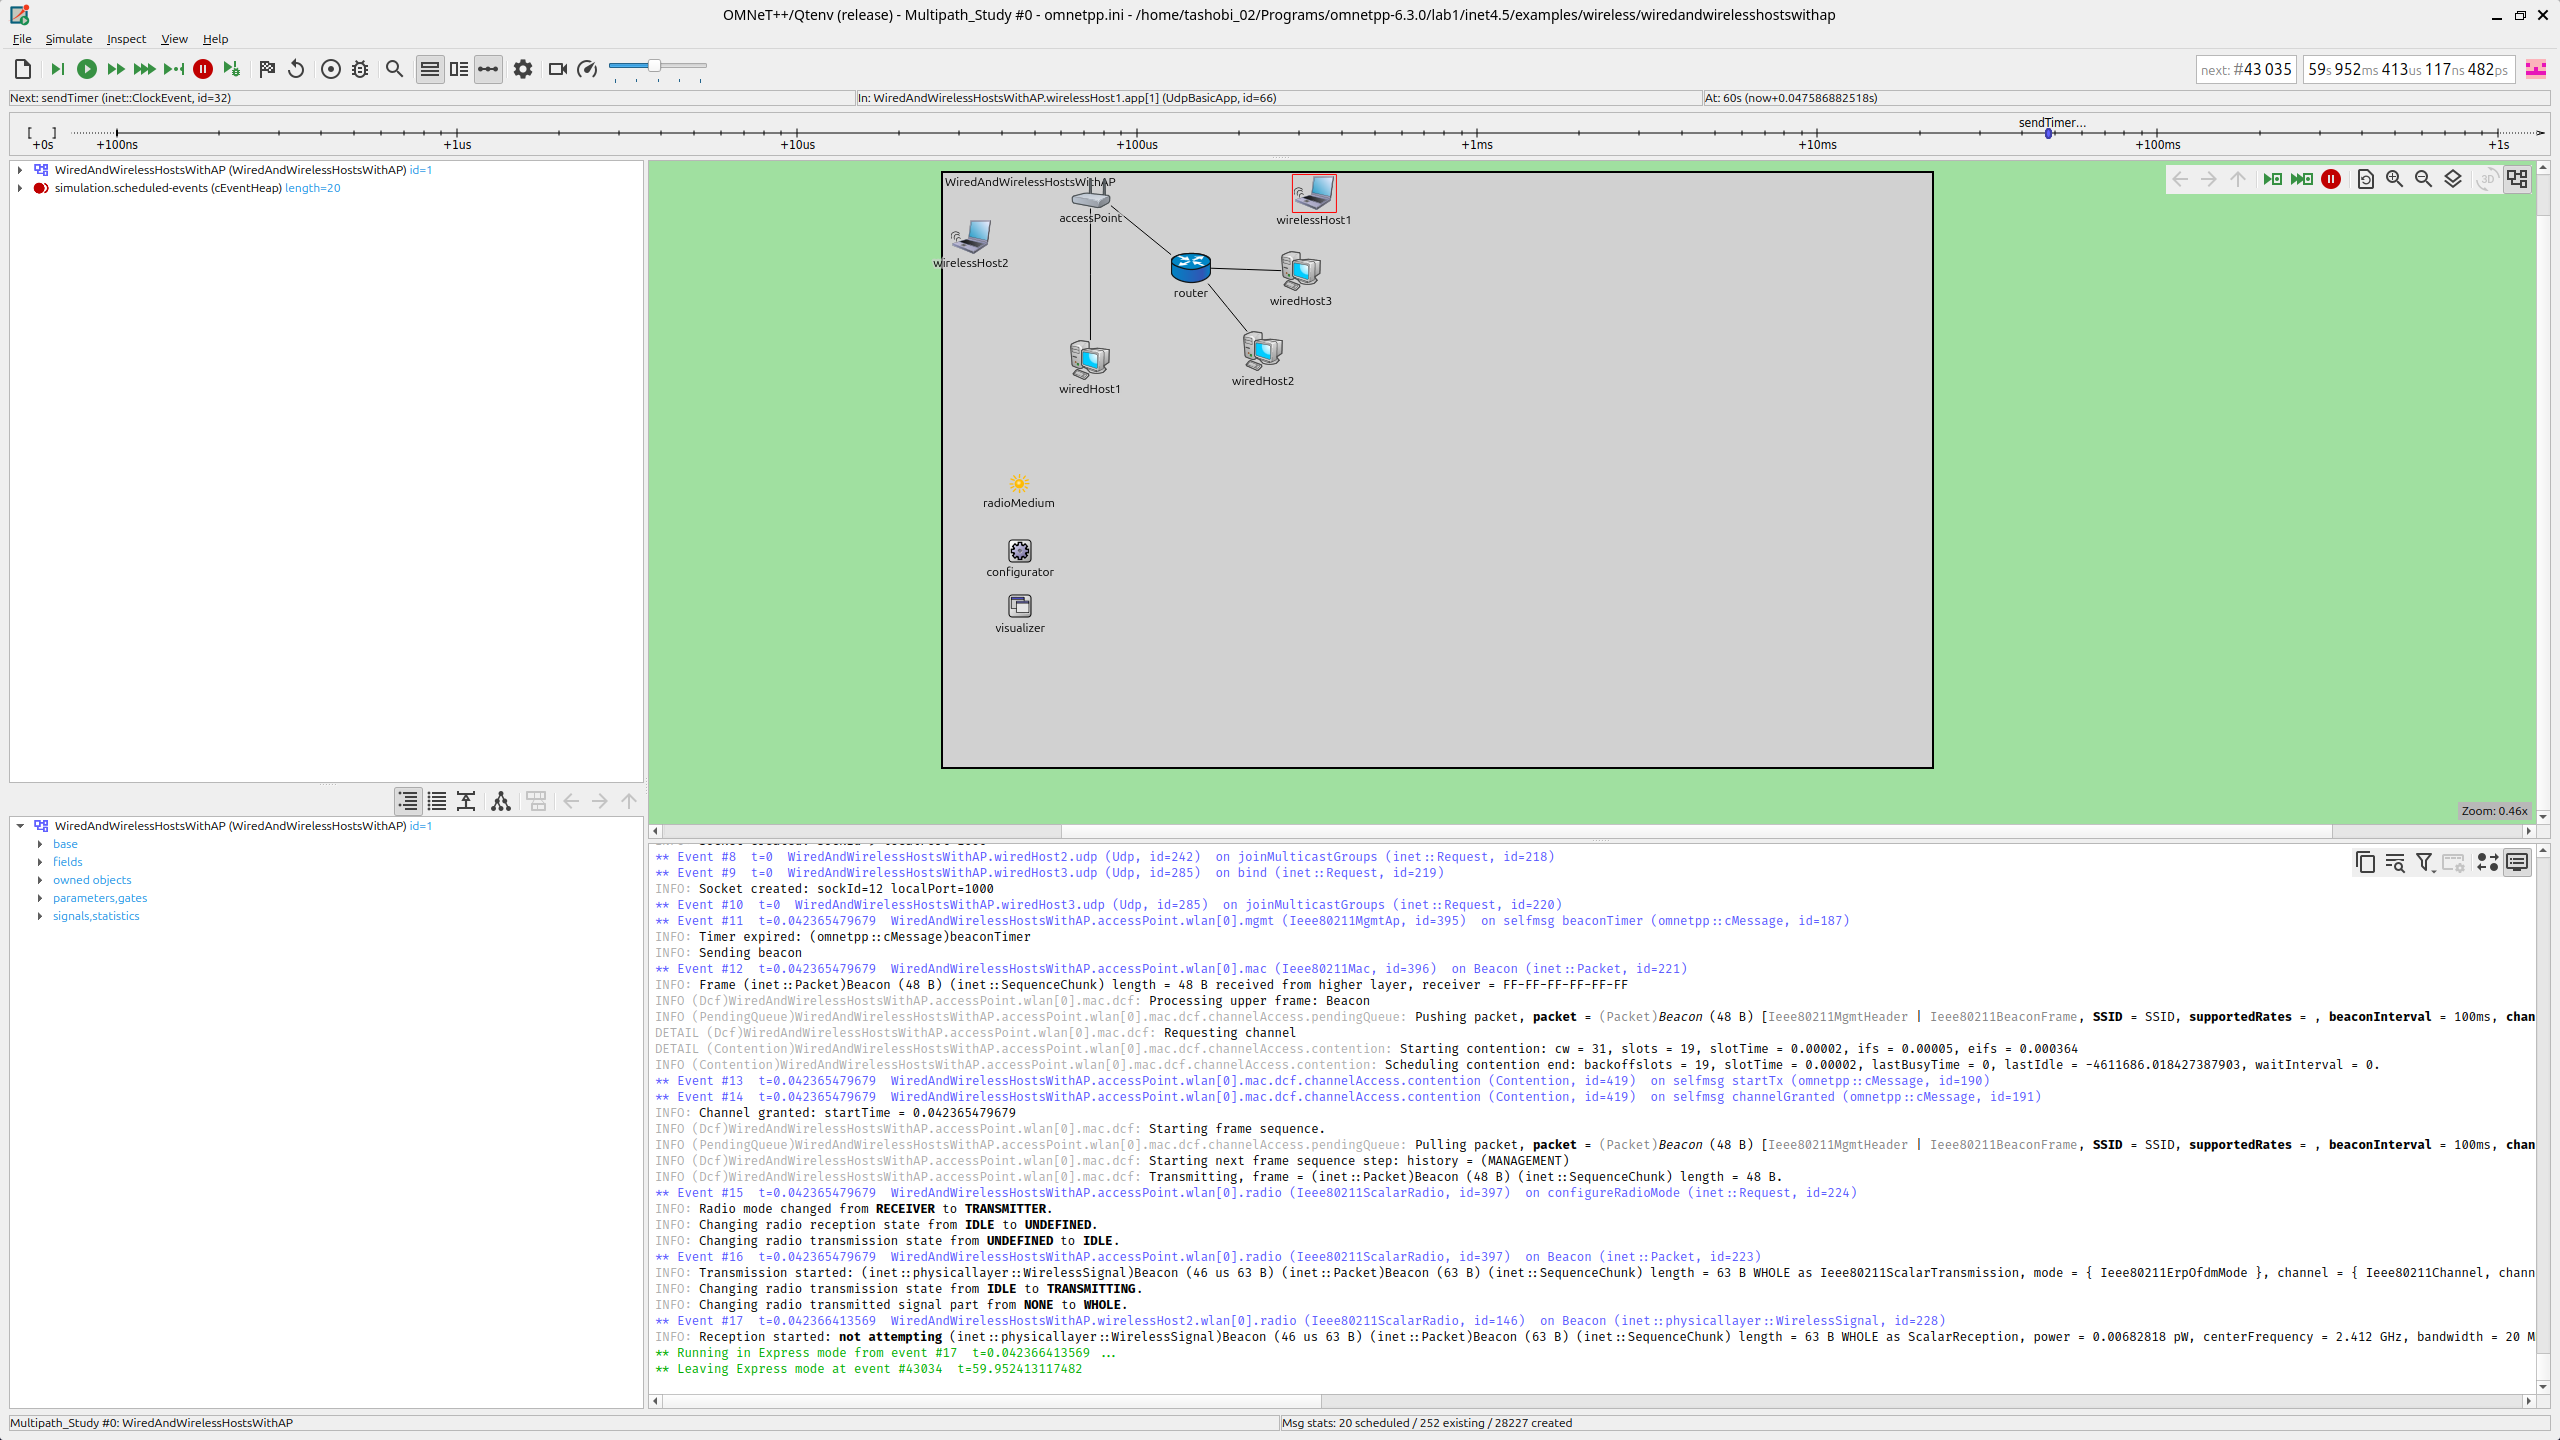
\includegraphics[width=\linewidth]{Figure/Task3_MultiPath_Study.png}
        \caption{Multipath\_Study ($\alpha = 3.5$) at $t \approx 60$\,s ---
                 visually identical to FreeSpace at these short node distances.}
    \end{subfigure}
    \vspace{6pt}
    \begin{subfigure}{0.9\linewidth}
        \centering
        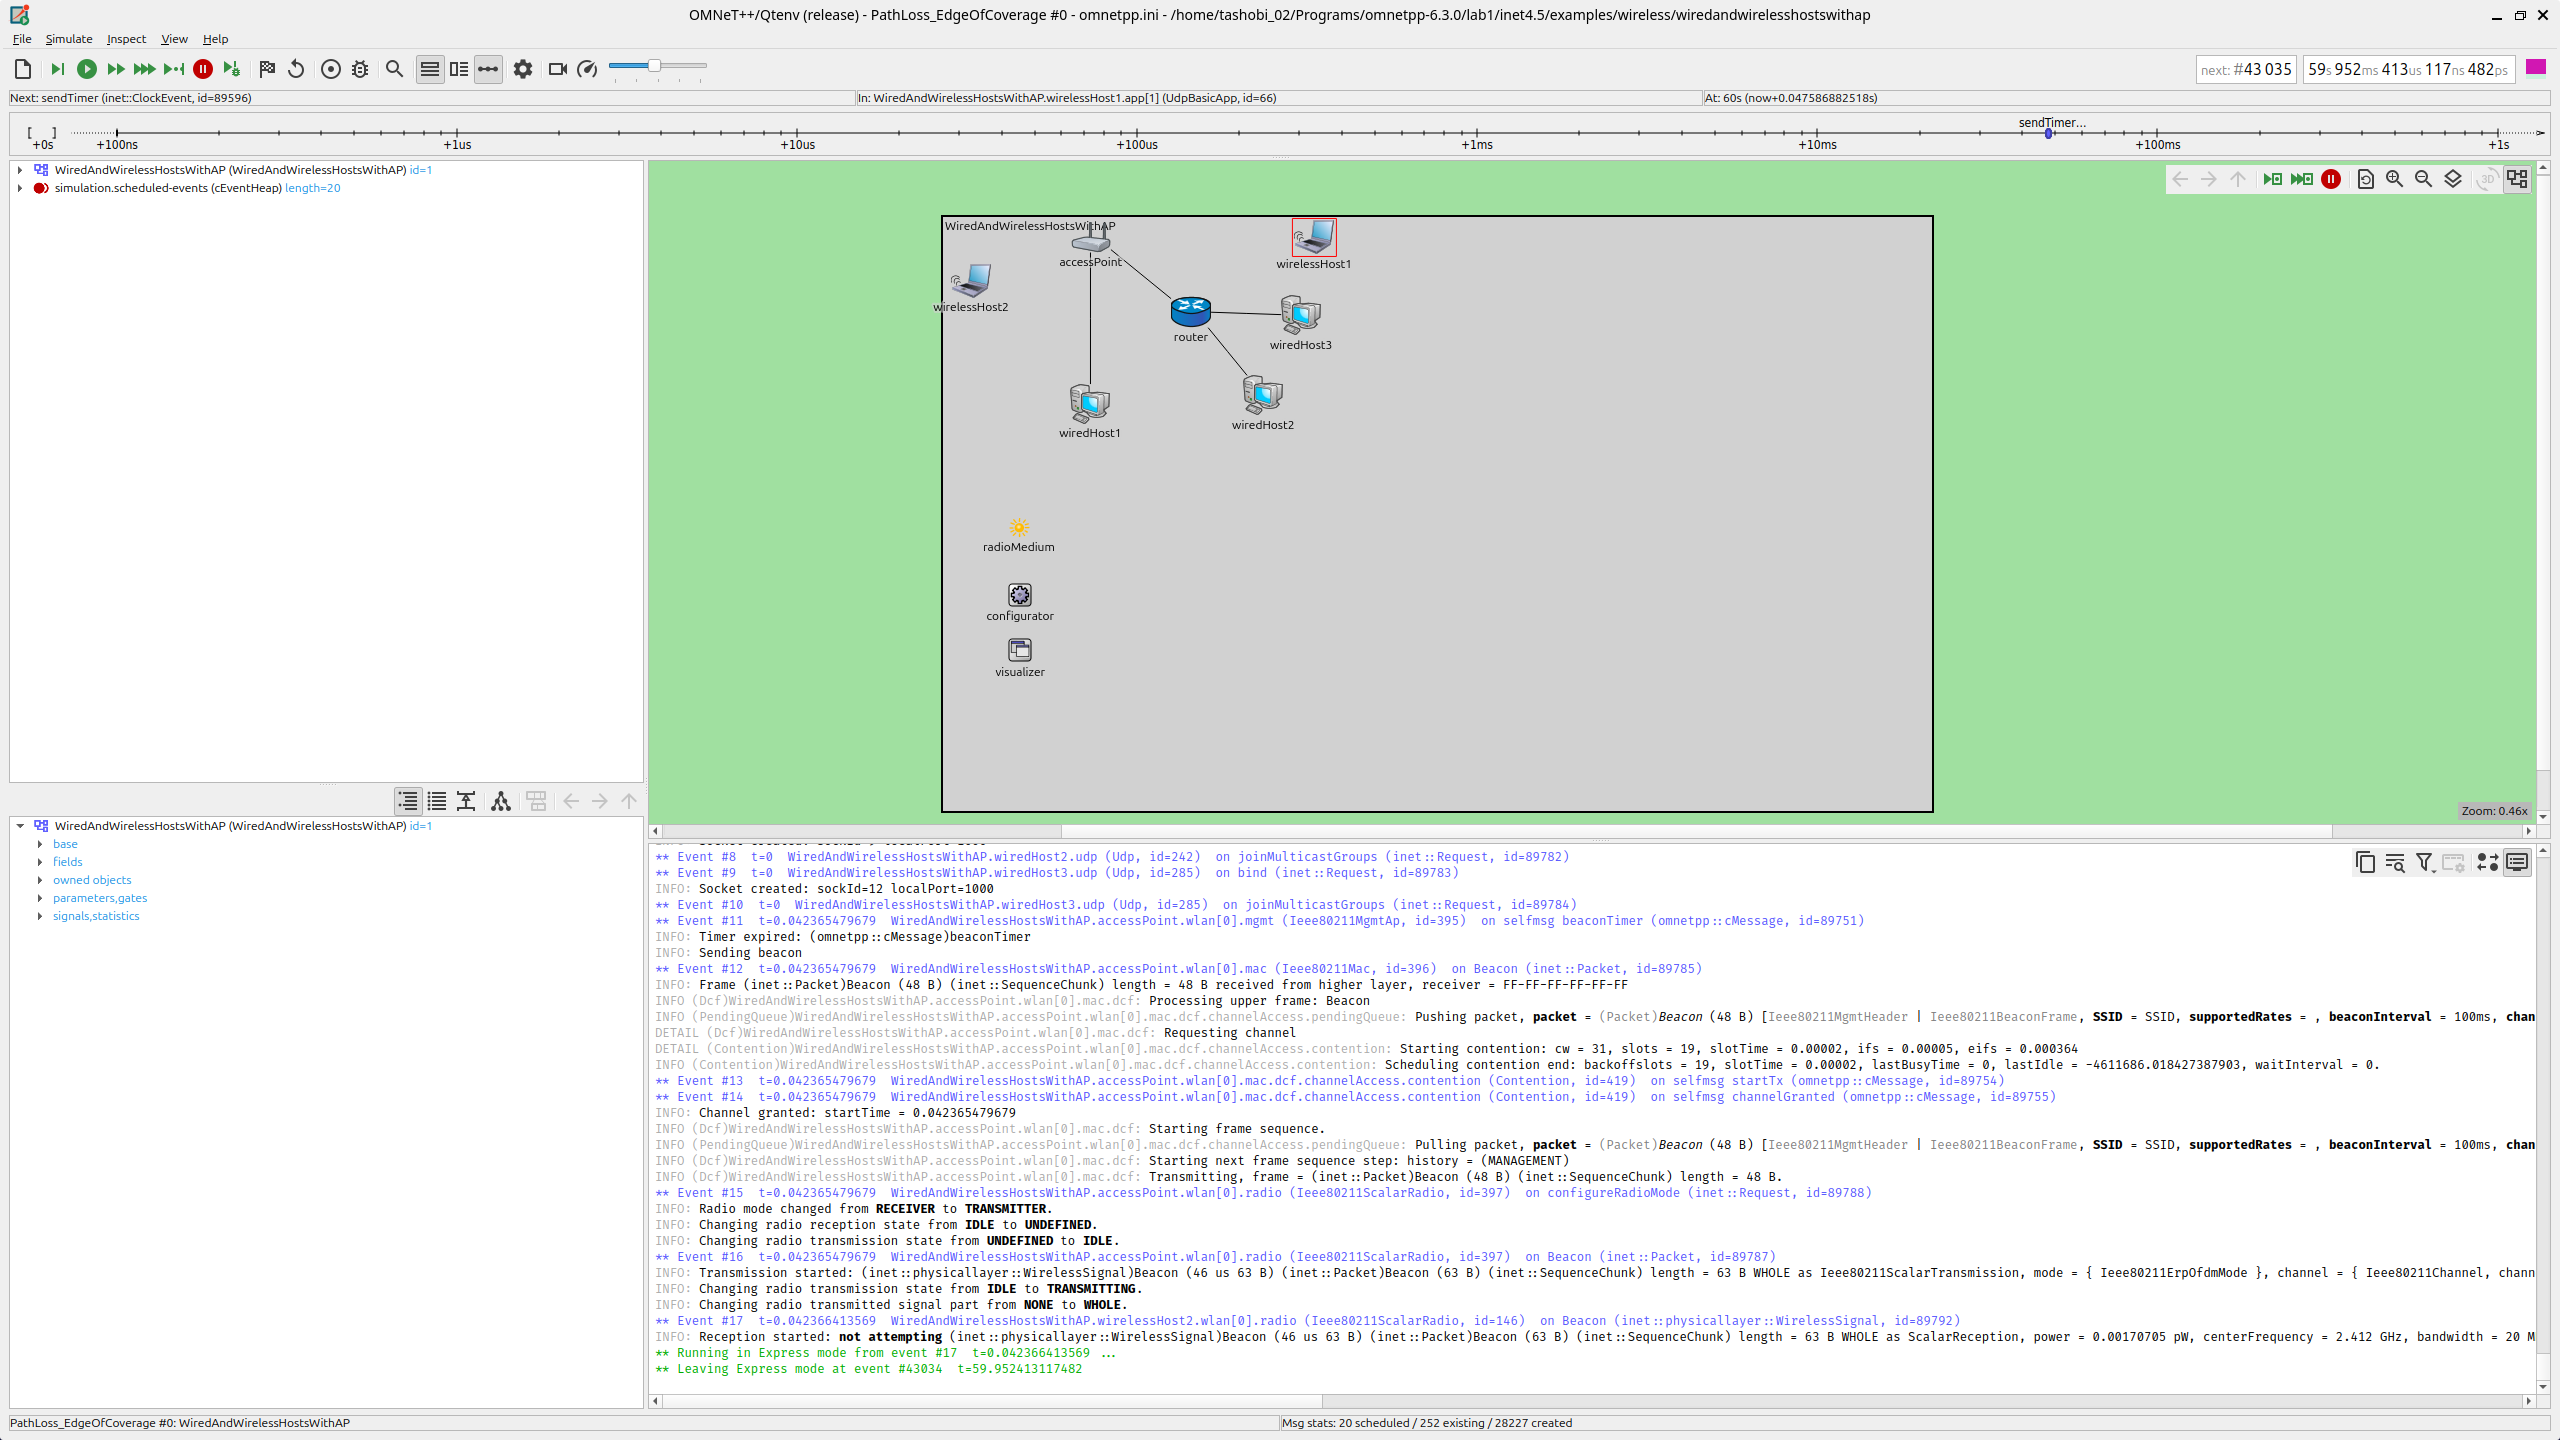
\includegraphics[width=\linewidth]{Figure/Task3_PathLoss_EdgeOfCoverage.png}
        \caption{PathLoss\_EdgeOfCoverage ($\alpha = 3.5$, 5\,mW) at
                 $t \approx 60$\,s --- complete wireless link failure; console
                 shows \textit{``Reception started: not attempting''} at
                 $\approx -118$\,dBm, far below $-85$\,dBm sensitivity.}
    \end{subfigure}
    \caption{Qtenv screenshots for Task 03.}
    \label{fig:task3}
\end{figure}

% ----------------------------------------------------------------
\subsection{Task 04: Co-Channel Interference --- NED + INI Extension}
% ----------------------------------------------------------------

\textbf{Background:} Wireless is a shared broadcast medium, and interference from
other sources is one of the main differences from wired networks described in
Lecture 1. This task models a 2.4\,GHz co-channel interferer that transmits
simultaneously with \texttt{wirelessHost1}, degrading the SINR at the access point
and reducing packet delivery.

\textbf{NED File Change:}
The submodule \texttt{interferer: WirelessHost} is added inside the
\texttt{submodules} block of the \texttt{WiredAndWirelessHostsWithAP} network,
positioned near \texttt{wirelessHost1} at \texttt{@display("p=62,210")}. No
explicit cable connection is required because the interferer joins the wireless
network automatically through the existing \texttt{radioMedium}.

\textbf{INI File Configurations:}
\begin{enumerate}
    \item \textbf{Interference\_Control:} The interferer node is present in the
          topology but configured with \texttt{numApps = 0} so it remains
          completely silent. Normal UDP communication runs between the wired
          and wireless hosts using baseline channel settings.

    \item \textbf{Interference\_Active:} Extends Interference\_Control. The
          interferer is activated with a \texttt{UdpBasicApp} that generates
          heavy traffic: 1400\,B packets at 0.05\,s intervals (20 packets/s),
          starting at $t = 20$\,s and stopping at $t = 140$\,s. This saturates
          the 2.4\,GHz channel and drives down the SINR seen by the access point
          when receiving \texttt{wirelessHost1}'s frames.
\end{enumerate}

\textbf{Observation Table:}
\begin{table}[H]
    \centering
    \small
    \renewcommand{\arraystretch}{1.3}
    \begin{tabularx}{\linewidth}{|l|c|X|X|}
        \hline
        \textbf{Phase} & \textbf{Time range}
            & \textbf{Control run}
            & \textbf{Active interference run} \\
        \hline
        Before interferer starts & $t = 0$--$20$\,s &
            Normal --- clean packet flow from \texttt{wirelessHost1} to AP &
            Normal --- identical to control; interferer is silent \\
        \hline
        During interference & $t = 20$--$140$\,s &
            Normal --- no interference present &
            Degraded / Failed --- \texttt{wirelessHost1}'s packet delivery
            drops sharply; SINR collapses as the interferer saturates the
            channel; many frames fail to decode at the AP \\
        \hline
        After interferer stops & $t = 140$--$180$\,s &
            Normal &
            Recovering to Normal --- SINR returns to the baseline level and
            \texttt{wirelessHost1}'s traffic resumes within a few seconds \\
        \hline
    \end{tabularx}
    \caption{Packet delivery observation table for Task 04.}
    \label{tab:task4_obs}
\end{table}

\textbf{Analysis Questions:}
\begin{enumerate}

    \item \textit{In Lecture 1 the SINR formula was given as
          $\mathrm{SINR} = S/(N+I)$. In the Interference\_Active run, which term
          changed compared to the control run? Did $S$ change? Explain.}

    \textbf{Answer:}
    Only the interference term \textbf{$I$} changed. The desired signal $S$ from
    \texttt{wirelessHost1} did not change: transmit power (20\,mW) and node
    positions remained the same, so the received signal power at the access point
    is identical in both runs. The background noise term $N$ also remained constant
    at $-110$\,dBm. The interferer adds additional signal energy on the same
    2.4\,GHz channel, increasing $I$ and therefore increasing the denominator
    $(N+I)$. This directly lowers the SINR and raises the BER for
    \texttt{wirelessHost1}'s transmissions, causing packet loss even though $S$
    itself is unchanged.

    \item \textit{After the interferer stopped at $t = 140$\,s, did
          \texttt{wirelessHost1}'s traffic recover? How long did recovery take?
          What does this tell us about co-channel interference vs.\ permanent
          noise?}

    \textbf{Answer:}
    Yes, \texttt{wirelessHost1}'s traffic recovered after the interferer stopped
    at $t = 140$\,s. Recovery is rapid --- typically within 1--5 simulated
    seconds --- because the CSMA/CA MAC layer immediately detects a quieter
    channel and resumes normal contention and backoff. This demonstrates that
    co-channel interference is \textbf{temporary and source-dependent}: once the
    interfering device ceases transmission, the full link budget is restored and
    the channel heals without any reconfiguration. By contrast, a raised
    permanent noise floor (as in Task 02) cannot be removed by waiting; the
    degradation persists for the entire simulation regardless of the traffic
    pattern.

    \item \textit{From Lecture 1, the ISM band (2.4\,GHz) is used by Wi-Fi,
          Bluetooth, microwave ovens, and cordless phones. Which real-world device
          does your interferer most closely represent, and why?}

    \textbf{Answer:}
    The interferer most closely models a \textbf{2.4\,GHz cordless phone}. Like
    the simulated interferer, a cordless phone has a defined start time (when a
    call begins) and a defined stop time (when the call ends), and it transmits
    continuously on the same 2.4\,GHz band throughout its active period. Lecture 1
    explicitly cites the example of a 2.4\,GHz wireless phone interfering with an
    802.11b network. A microwave oven, by contrast, is better modelled by raised
    background noise (as in Noise\_Extreme in Task 02) because it generates
    wideband, non-802.11-formatted electromagnetic noise rather than coherent
    frames that contend on the channel.

    \item \textit{Propose one practical solution from Lecture 1 that a network
          engineer could use to reduce this interference. Explain how it addresses
          the problem.}

    \textbf{Answer:}
    The most effective solution is \textbf{adaptive frequency selection} --- moving
    the Wi-Fi network to the 5\,GHz band (IEEE 802.11a/n/ac/ax) or selecting a
    non-overlapping 2.4\,GHz channel (channels 1, 6, or 11). Lecture 1 lists
    ``adaptive frequency selection and smart AP placement'' as countermeasures for
    interference. This solution addresses the root cause: the interferer and the
    victim share the same radio frequency, so their signals overlap at the access
    point and degrade SINR. By moving to a different frequency, $I$ returns to zero
    in the SINR formula regardless of how heavily the interferer transmits,
    restoring full link quality.

\end{enumerate}

% --- Figures ---
\begin{figure}[H]
    \centering
    \begin{subfigure}{0.9\linewidth}
        \centering
        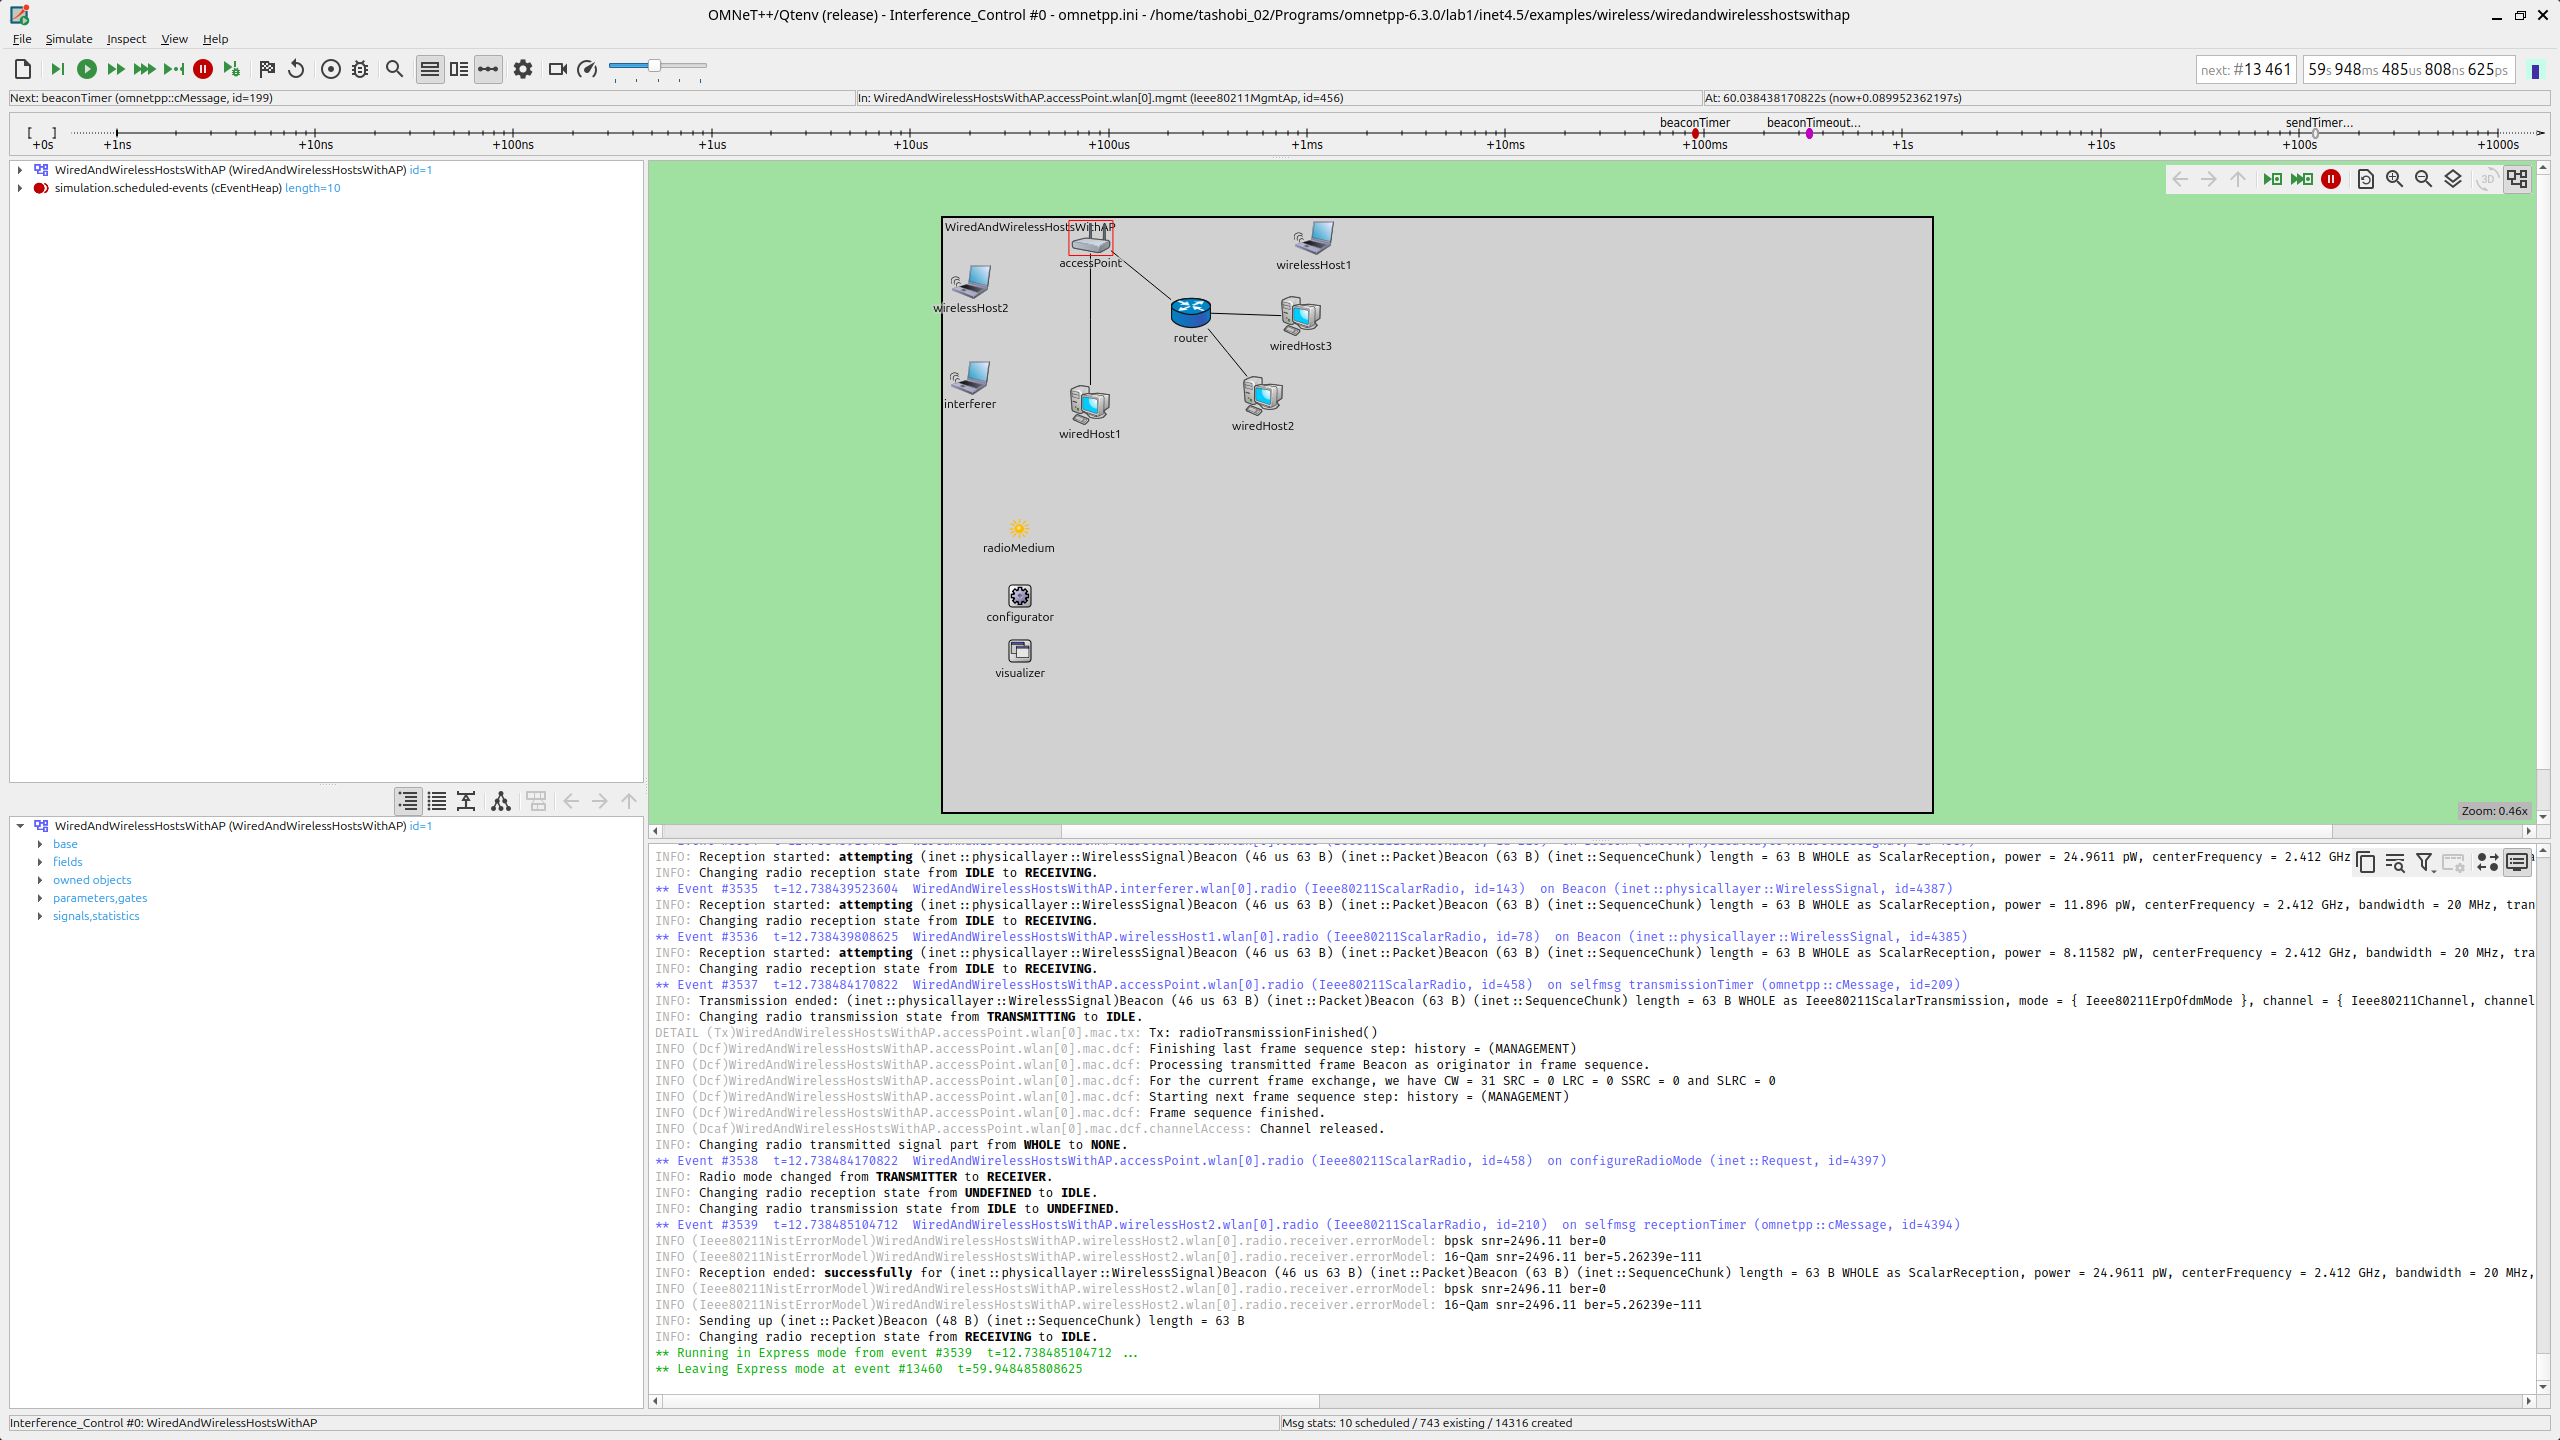
\includegraphics[width=\linewidth]{Figure/Task4_InterferenceControl.png}
        \caption{Interference\_Control at $t \approx 60$\,s --- interferer is
                 present but silent; \texttt{wirelessHost1} traffic flows
                 normally.}
    \end{subfigure}
    \vspace{6pt}
    \begin{subfigure}{0.9\linewidth}
        \centering
        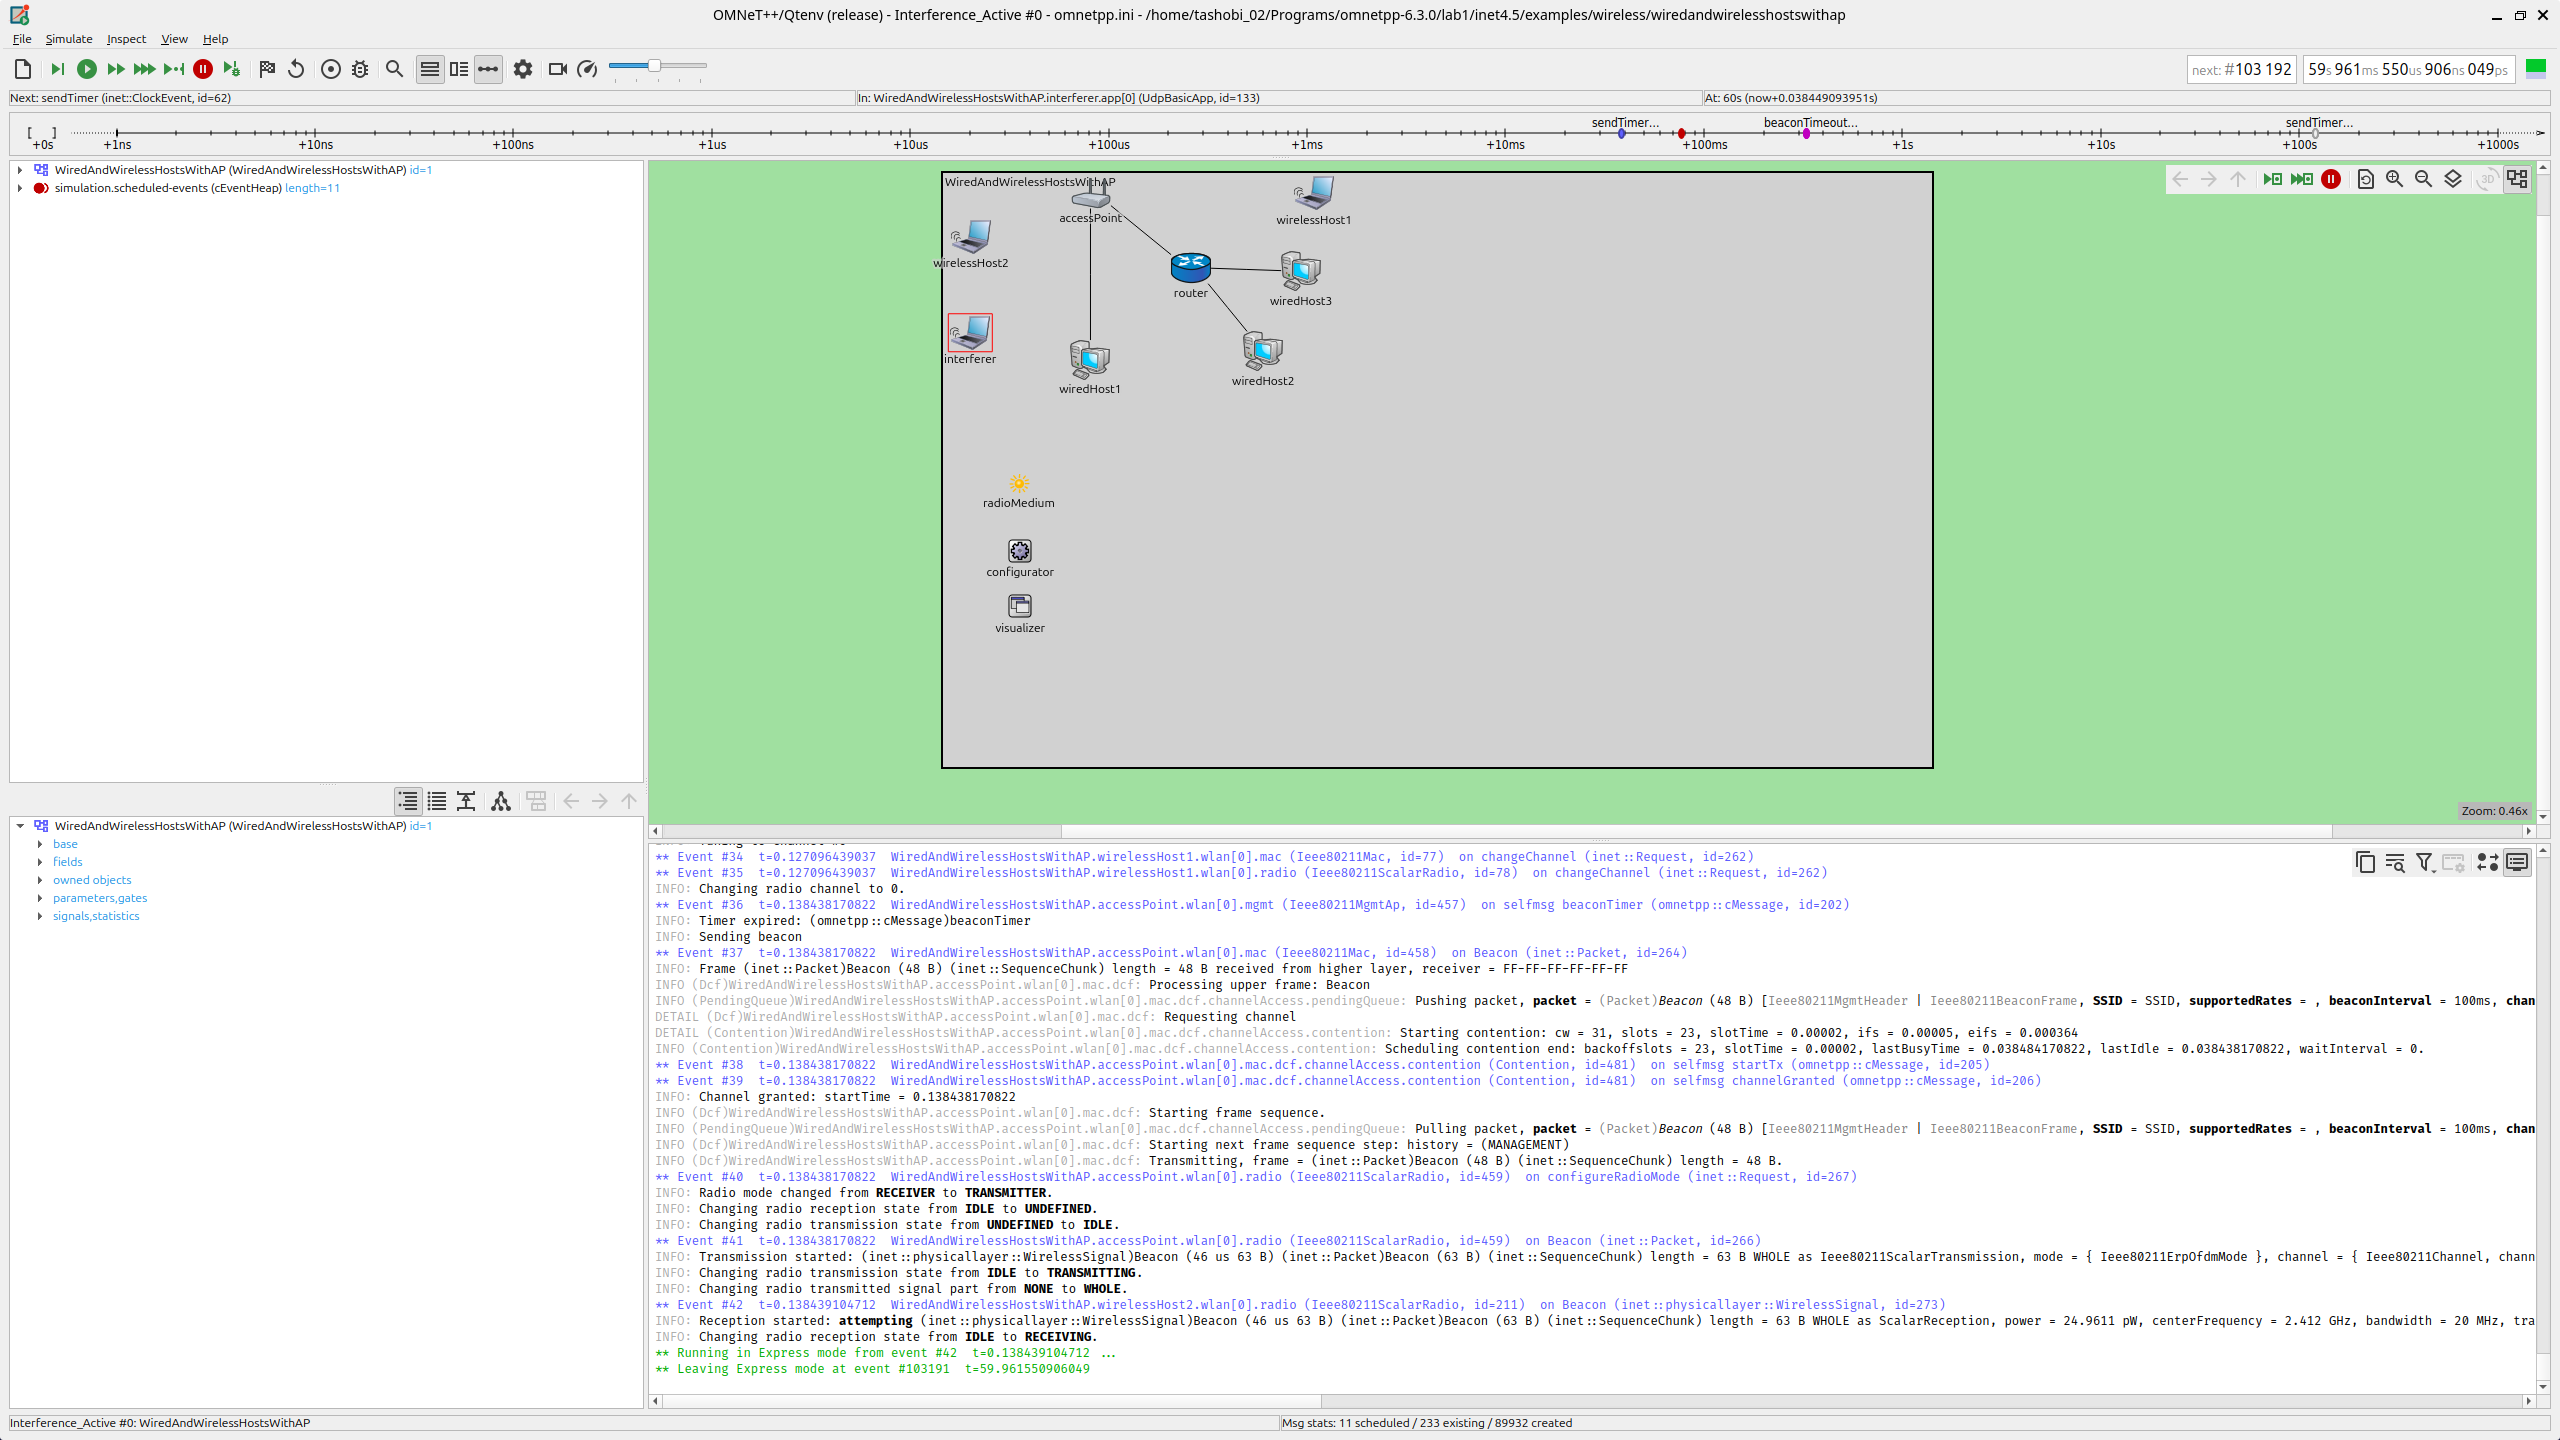
\includegraphics[width=\linewidth]{Figure/Task4_InterferenceActive.png}
        \caption{Interference\_Active at $t \approx 60$\,s --- interferer is
                 transmitting heavily; SINR at the AP is degraded and
                 \texttt{wirelessHost1}'s packet delivery drops.}
    \end{subfigure}
    \vspace{6pt}
    \begin{subfigure}{0.9\linewidth}
        \centering
        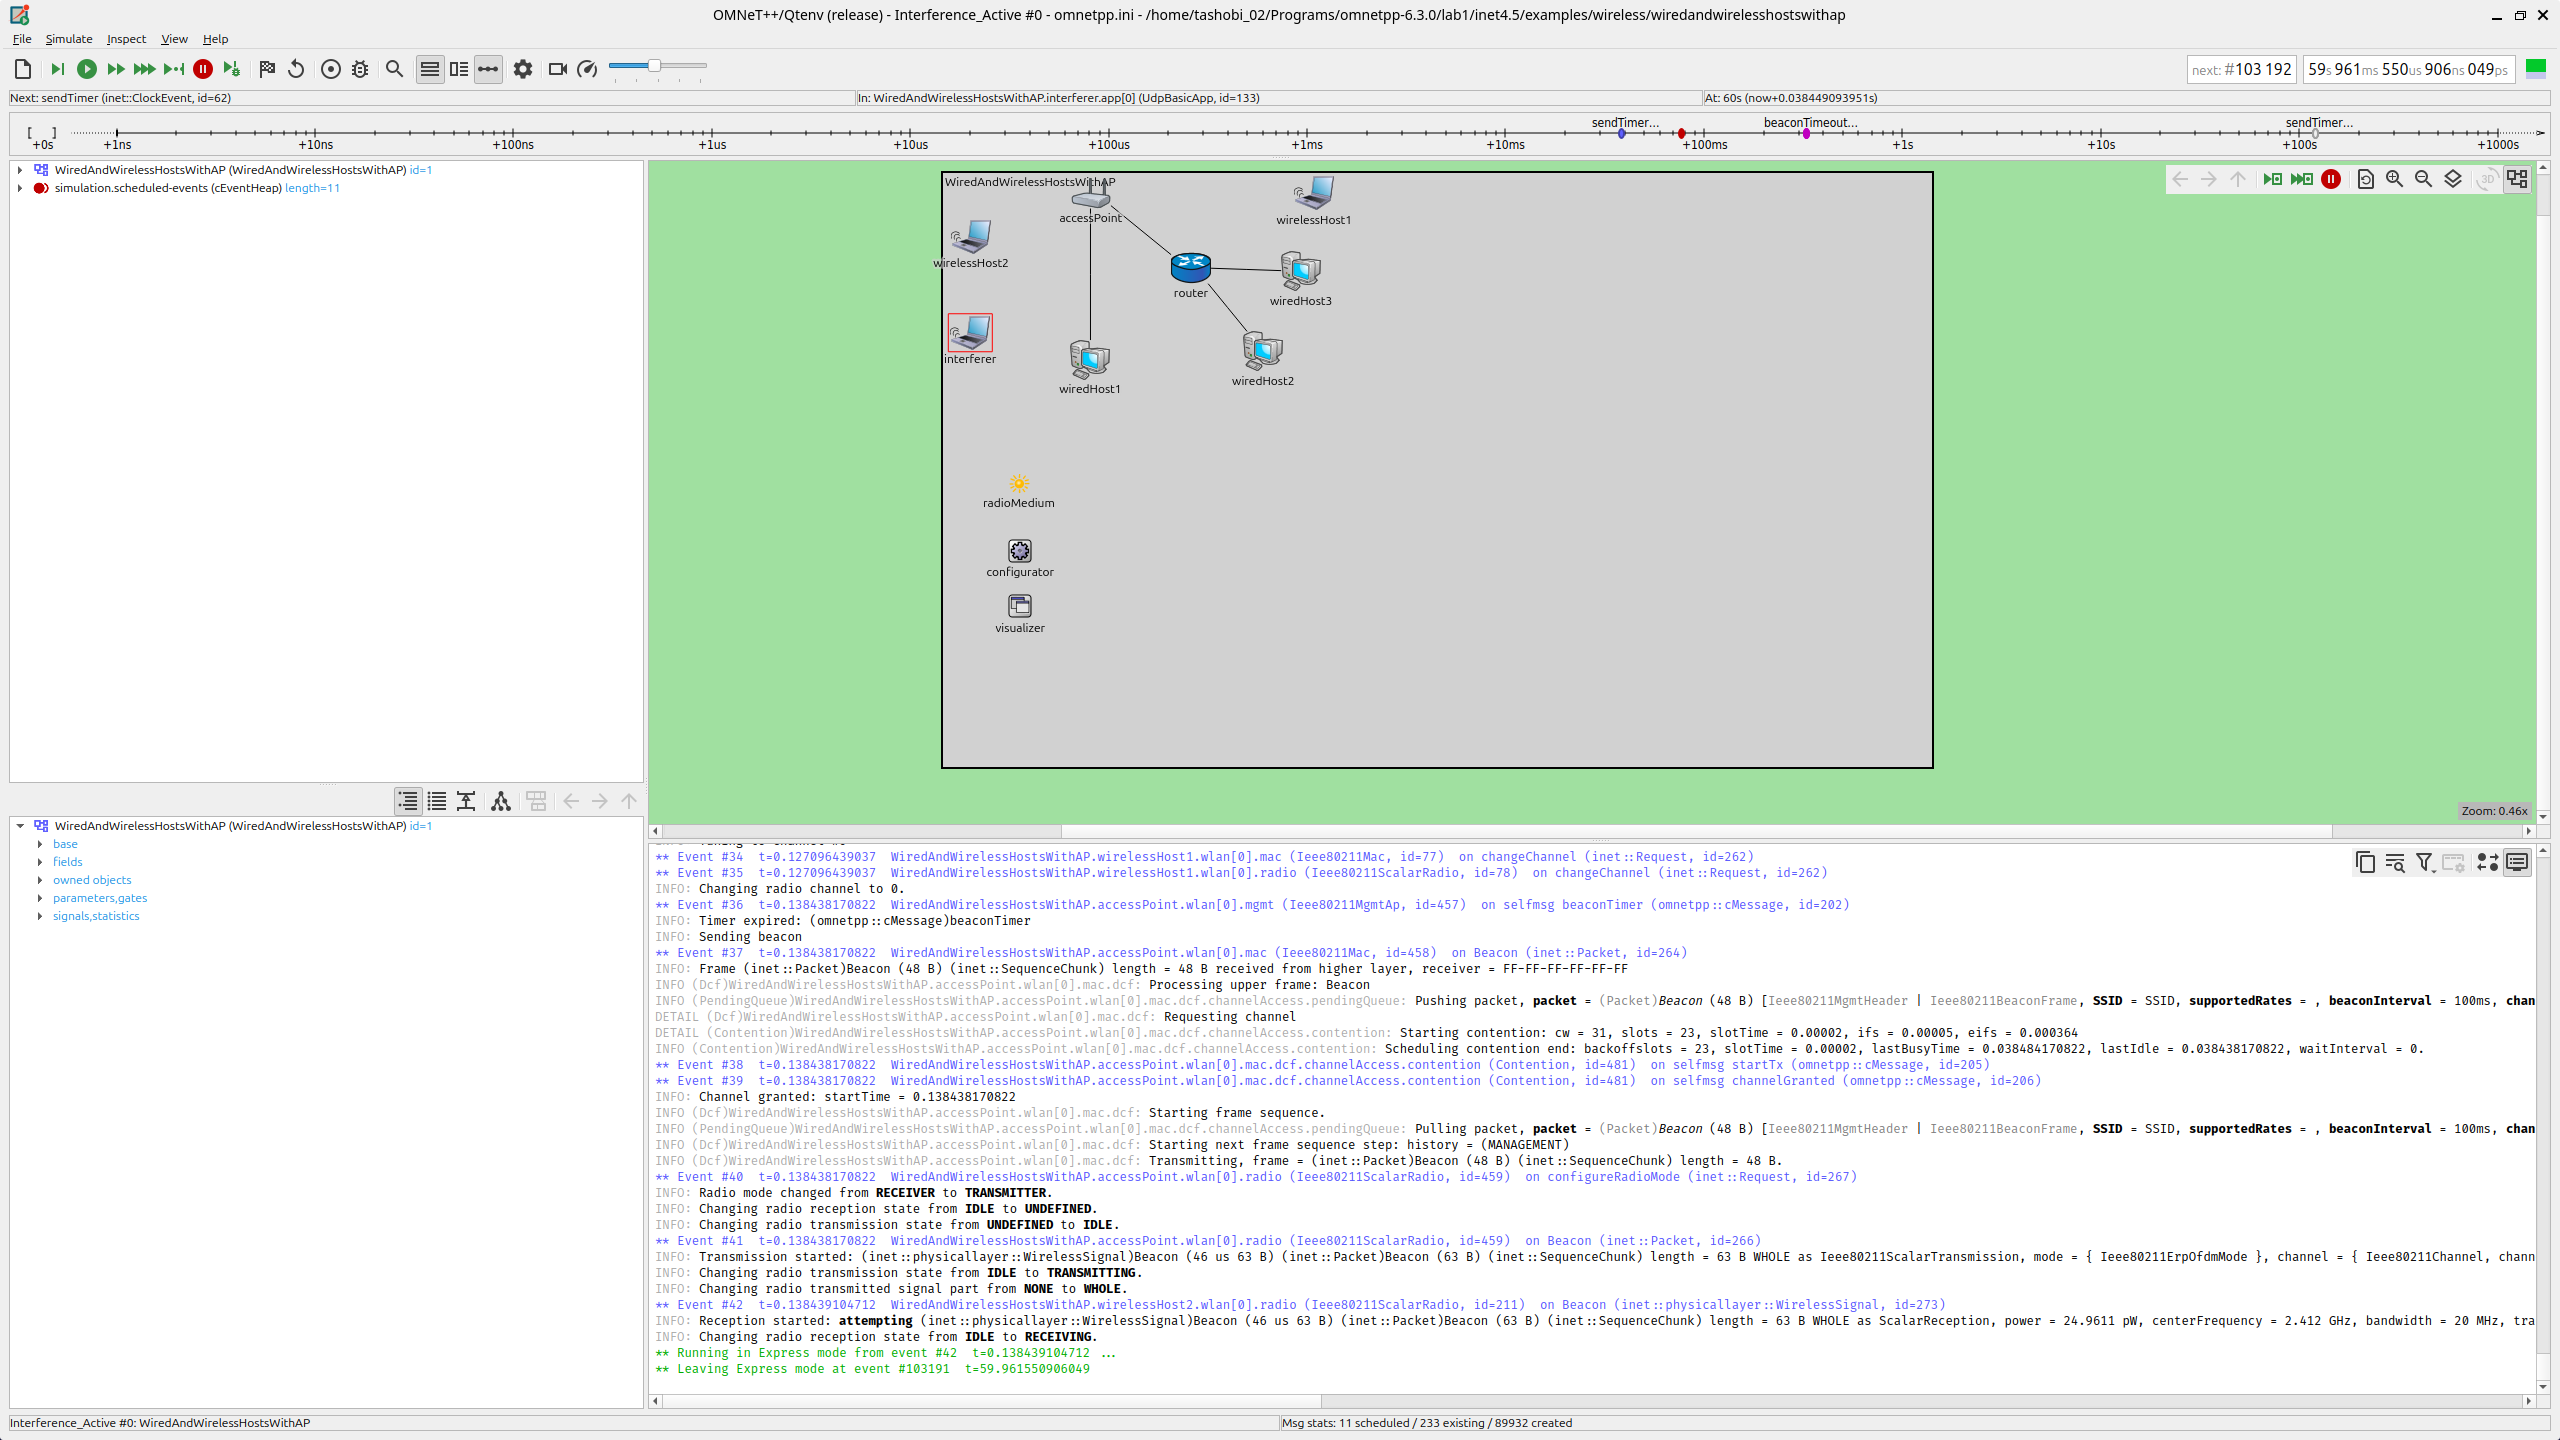
\includegraphics[width=\linewidth]{Figure/Task4_InterferenceActive.png}
        \caption{Interference\_Active at $t \approx 150$\,s (recovery phase) ---
                 the interferer stopped at $t = 140$\,s; \texttt{wirelessHost1}'s
                 traffic is returning to normal.
                 \textit{Note: a dedicated recovery screenshot taken at
                 $t \approx 150$\,s should replace this image.}}
    \end{subfigure}
    \caption{Qtenv screenshots for Task 04.}
    \label{fig:task4}
\end{figure}

\end{document}